% ======================================================================
% Relatório Final de Iniciação Científica — UFABC
% Tema: Iridologia sob Lentes Científicas: Avaliação Crítica com ML
% ======================================================================

\documentclass[11pt,a4paper]{article}
\usepackage{graphicx}
% ---------------------- Pacotes ----------------------
\usepackage[utf8]{inputenc}
\usepackage[T1]{fontenc}
\usepackage[portuguese]{babel}

\usepackage{setspace}
\usepackage{geometry}
\usepackage{tabularx}
\geometry{a4paper, top=2.5cm, bottom=2cm, left=2.5cm, right=2.5cm}

\usepackage{graphicx}
\graphicspath{{./imagens/}}
\usepackage{float}

\usepackage{amsmath, amssymb}
\usepackage{siunitx}
\sisetup{
  mode = match,
  propagate-math-font = true,
  reset-math-version = false,
  reset-text-family = false,
  reset-text-series = false,
  reset-text-shape = false,
  text-family-to-math = true,
  text-series-to-math = true
}

\usepackage{booktabs}
\usepackage{multirow}
\usepackage{array}

% Gráficos vetoriais nativos (TikZ/pgfplots)
\usepackage{pgfplots}
\pgfplotsset{compat=1.18}
\pgfplotsset{/pgf/number format/use comma}
\usepgfplotslibrary{colormaps}
\usepgfplotslibrary{polar}
\usetikzlibrary{backgrounds}
\usepackage{comment}
\usepackage{textcomp} % \textdegree nas legendas polares

% Espaçamento compacto ao redor de floats e legendas
\setlength{\textfloatsep}{8pt plus 2pt minus 2pt}
\setlength{\intextsep}{8pt plus 2pt minus 2pt}
\setlength{\abovecaptionskip}{4pt}
\setlength{\belowcaptionskip}{2pt}

% Listas compactas (padrão acadêmico, menos espaço vertical)
\usepackage{enumitem}
\setlist{topsep=2pt, itemsep=1pt, parsep=0pt}

\usepackage{fancyhdr}
\setlength{\headheight}{14pt}

% Natbib em autor--ano (compatível com \bibitem[Autor(ano)]{...})
\usepackage[authoryear, round, sort]{natbib}

% hyperref por último (boa prática)
\usepackage[bookmarks=true, colorlinks=true, linkcolor=blue, citecolor=blue, urlcolor=blue]{hyperref}

\usepackage{indentfirst}
\setlength{\parindent}{1.25cm}
\setlength{\parskip}{0.2cm}
% Absorve pequenos estouros de linha (overfull hboxes) sem afetar o restante
\setlength{\emergencystretch}{1em}

% ---------------------- Cabeçalho/Rodapé ----------------------
\pagestyle{fancy}
\fancyhf{}
\lhead{\small UFABC — Programa de Iniciação Científica}
\rhead{\small Relatório Final de Iniciação Científica}
\cfoot{\thepage}

% ---------------------- Metadados ----------------------
\title{\textbf{Relatório Final de Iniciação Científica}\\
\large Iridologia sob Lentes Científicas: Avaliação Crítica com Aprendizado de Máquina\\
\vspace{0.2cm}\normalsize (Ênfase: alegações diagnósticas para diabetes mellitus tipo 2)}
\date{Santo André, 10 de março de 2026}

% ----------------------------------------------------------------------
\begin{document}

\hypersetup{pageanchor=false}

% ====================== Capa (modelo CPIC — timbre UFABC) ======================
\begin{titlepage}
\centering

% Timbre / cabeçalho oficial da UFABC
\IfFileExists{imagens/logo_ufabc.png}{%
    \noindent
\includegraphics[width=\textwidth]{logo_ufabc.png}%
}{%
    \noindent\fbox{\parbox{\dimexpr\textwidth-2\fboxsep-2\fboxrule}{%
        \centering\vspace{0.8cm}[\,timbre da UFABC em \texttt{imagens/logo\_ufabc.png}\,]\vspace{0.8cm}}}%
}

\vspace{1.5cm}

{\normalsize \textbf{Relatório Final de Iniciação Científica referente ao Edital: 01/2025}}\\[1.5cm]

\raggedright
\normalsize
\textbf{Nome do aluno:} Vinicius Sedrim.\\[1.5cm]
\textbf{Assinatura do aluno:} \rule{7.5cm}{0.4pt}\\[0.45cm]
\textbf{Nome do orientador:} Vladimir Emiliano Moreira Rocha.\\[1.5cm]
\textbf{Assinatura do orientador:} \rule{6.5cm}{0.4pt}\\[0.45cm]
\textbf{Título do projeto:} Iridologia sob Lentes Científicas: Avaliação Crítica com Aprendizado de Máquina.\\[0.45cm]
\textbf{Palavras-chave do projeto:} Iridologia; Medicina Alternativa; Visão Computacional; Aprendizado de Máquina.\\[0.45cm]
\textbf{Área do conhecimento do projeto:} Ciência da Computação.\\[0.45cm]
\textbf{Bolsista:} Sim. CNPq.\\

\vfill
\begin{center}
{\normalsize Santo André}\\
{\normalsize \today}
\end{center}
\end{titlepage}

% ====================== Resumo ======================
\begin{abstract}
Este projeto conduz uma \textbf{avaliação crítica, científica e reprodutível} de alegações de que padrões observáveis na íris possam sustentar inferência de \textbf{diabetes mellitus tipo 2 (DM2)}, no contexto da literatura de iridologia e de estudos recentes em \textit{machine learning} (ML). Estudos clínicos clássicos e revisões sistemáticas relatam \textbf{baixa acurácia} e \textbf{baixa confiabilidade} da iridologia quando avaliada sob protocolos controlados. Em contraste, trabalhos em ML frequentemente reportam alto desempenho ao classificar DM2 a partir de imagens da íris, porém com limitações metodológicas recorrentes, incluindo amostras reduzidas, heterogeneidade de protocolos, risco de \textit{data leakage} (inclusive por identidade) e ausência de testes sistemáticos de robustez.

Neste relatório, descrevem-se o problema, os objetivos, a base teórica e uma \textbf{metodologia auditável} orientada à \textbf{generalização} e ao \textbf{controle de viés}. O protocolo emprega: (i) particionamento \textit{person-based} (separação por indivíduo) para mitigar vazamento por identidade; (ii) validação cruzada estratificada e reexecução completa do \textit{pipeline} (segmentação, normalização e classificação); (iii) avaliação por múltiplas métricas (Acc, Sens, Esp, Prec e F1); (iv) análises de estabilidade sob reamostragens/\textit{folds} e diferentes sementes; e (v) testes de sensibilidade a transformações fotométricas. Os resultados obtidos indicam desempenho elevado e consistente em diferentes classificadores sob controle \textit{person-based}, com manutenção do desempenho sob perturbações fotométricas moderadas. Análises locais (setores angulares e ROI pancreática em malha \(12\times 12\)) são tratadas como \textbf{exploratórias} e interpretadas como \textbf{hipóteses candidatas}, cuja validade exige verificação confirmatória com controles para múltiplas comparações e testes adicionais de generalização.
\end{abstract}


\tableofcontents
\newpage

\hypersetup{pageanchor=true}
\pagenumbering{arabic}
\setcounter{page}{1}

\singlespacing

% ====================== Introdução ======================
\section{Introdução}
A iridologia é uma prática que afirma ser possível identificar indícios de saúde e doença a partir de padrões observáveis na íris, como variações de textura, coloração, sulcos, anéis e marcas. Em sua forma mais difundida, utiliza \textit{mapas iridológicos} que associam regiões específicas do olho a órgãos e sistemas do corpo, sugerindo que alterações locais na íris poderiam refletir disfunções internas \citep{Ernst2000ArchOphthalmol}. Por isso, em alguns contextos, a iridologia é apresentada como proposta complementar de triagem e acompanhamento. Entretanto, quando a prática é apresentada com finalidade \textbf{diagnóstica} (isto é, para inferir doenças de forma confiável), a exigência científica é alta: é necessário demonstrar validade, reprodutibilidade, controle de vieses e desempenho consistente em cenários realistas \citep{AusGovIridology2025}.

Essa exigência se torna ainda mais crítica ao considerar doenças crônicas de grande impacto, como o diabetes mellitus tipo 2 (DM2). O DM2 é uma condição metabólica multifatorial associada a complicações cardiovasculares, renais, neurológicas e oftalmológicas, e cuja progressão pode permanecer silenciosa por longos períodos \citep{WHOdiabetes2024}. Por esse motivo, estratégias de detecção precoce e monitoramento são frequentemente discutidas em saúde pública, especialmente quando envolvem soluções de baixo custo e fácil acesso \citep{WHOdiabetes2024}. Nesse cenário, propostas não invasivas naturalmente ganham espaço --- incluindo ideias que vão desde marcadores fisiológicos validados até hipóteses que ainda carecem de evidência clínica robusta.

A literatura médica clássica, no entanto, apresenta resultados desfavoráveis à iridologia quando avaliada sob protocolos controlados e com critérios diagnósticos objetivos. Estudos clínicos e revisões sistemáticas relatam baixa acurácia e pouca confiabilidade, sugerindo que a prática não sustenta promessas diagnósticas em condições investigadas \citep{Simon1979JAMA, Knipschild1988BMJ, Ernst2000ArchOphthalmol}. Em linha semelhante, avaliações recentes que sintetizam evidências para decisões de saúde pública reforçam a ausência de confiabilidade diagnóstica atribuível à iridologia \citep{AusGovIridology2025}. Esses resultados não apenas questionam a validade do método, mas também indicam um risco prático: interpretações incorretas podem gerar falsa segurança, ansiedade desnecessária ou atraso em diagnóstico clínico adequado.

Paralelamente, o avanço recente de visão computacional e aprendizado de máquina (\textit{machine learning}, ML) introduz um elemento novo nesse debate. Modelos modernos são capazes de aprender padrões complexos e sutis, com frequência imperceptíveis a observadores humanos, o que reabre uma questão central: existe algum sinal estatístico real nas imagens associado ao DM2? Ou, alternativamente, desempenhos elevados reportados por modelos decorrem de atalhos e artefatos do processo experimental, como diferenças de iluminação e câmera, ruídos de segmentação ou vazamento de dados (\textit{data leakage}), que permitem ao modelo reconhecer identidade (ou características indiretas) em vez de doença \citep{SamantAgarwal2018CMPB}? Assim, métricas altas podem refletir confundidores do \textit{pipeline} e do protocolo de aquisição, e não necessariamente a aprendizagem de um marcador clínico.

Este projeto situa-se precisamente nesse ponto de tensão: de um lado, uma prática historicamente contestada por estudos clínicos; de outro, resultados em ML que sugerem separabilidade entre grupos (indivíduos com DM2 versus indivíduos controle) \citep{SamantAgarwal2018CMPB}. O objetivo não é confirmar crenças prévias, mas construir um protocolo experimental rigoroso e auditável que permita testar \textbf{as hipóteses típicas de mapeamentos iridológicos} de forma justa. Para isso, adota-se um \textit{pipeline} reprodutível (segmentação, normalização e validação estratificada), métricas completas (incluindo sensibilidade e especificidade) e controles explícitos contra vazamento de dados --- em especial vazamento por identidade, por meio de separação por indivíduo nos particionamentos. Além disso, realizam-se análises locais por região, conectando os experimentos às hipóteses espaciais propostas por mapeamentos iridológicos. Assim, busca-se diferenciar evidência de sinal estatístico de explicações alternativas baseadas em viés metodológico e artefatos, produzindo uma conclusão baseada em resultados replicáveis e critérios de generalização.


% ====================== Problema de Pesquisa ======================
\section{Problema e Questões de Pesquisa}

\subsection{Contexto e motivação do problema}
Como discutido na Introdução, a iridologia pressupõe que a íris conteria marcas reveladoras de condições sistêmicas --- hipótese que a literatura clínica clássica não sustenta sob protocolos controlados \citep{Simon1979JAMA, Knipschild1988BMJ, Ernst2000ArchOphthalmol}. O aprendizado de máquina reabre parcialmente o debate, pois alguns estudos relatam acurácias elevadas para classificar DM2 a partir de imagens da íris \citep{SamantAgarwal2018CMPB}. Contudo, em visão computacional médica, desempenhos altos podem decorrer de fatores alheios a um marcador clínico legítimo: \textit{data leakage} (p.\ ex., o mesmo indivíduo em treino e teste), viés de aquisição (câmera, iluminação, ambiente), rotulagem imperfeita ou padrões introduzidos pela segmentação e normalização \citep{Zech2018}. Nesses casos, o modelo aprende \textbf{atalhos estatísticos} (\textit{shortcuts}) válidos apenas no conjunto específico, sem generalização.

Dessa forma, o desafio científico central não consiste apenas em obter valores elevados de acurácia, mas em demonstrar que o desempenho observado apresenta propriedades fundamentais de validade empírica, a saber:
(i) é \textbf{reprodutível}, ou seja, mantém-se sob reexecuções do experimento;
(ii) é \textbf{generalizável}, isto é, resiste a novas divisões dos dados e, idealmente, a conjuntos independentes;
(iii) não depende predominantemente de fatores não clínicos, como artefatos e vieses metodológicos;
e (iv) permanece consistente quando hipóteses locais inspiradas por mapas iridológicos são avaliadas.

\subsection{Problema central}
O problema central deste projeto \textbf{não se limita a} obter valores elevados de acurácia: consiste em avaliar se imagens da íris contêm informação diagnóstica útil para o DM2 quando analisadas sob protocolo rigoroso --- com controle explícito de vieses e prevenção de \textit{data leakage} --- e se o desempenho observado é reprodutível, robusto e generalizável. Em outras palavras, busca-se determinar se a separabilidade entre indivíduos com DM2 e controles reflete um sinal estatístico consistente ou se é melhor explicada por limitações do desenho experimental e artefatos metodológicos.

\subsection{Questões específicas}
As questões de pesquisa que operacionalizam esse problema central são formuladas nos seguintes termos:

\begin{enumerate}
    \item \textbf{Validade global do sinal (íris inteira):} verificar se, ao aplicar um \textit{pipeline} reprodutível (segmentação, normalização e extração de representações) e treinar modelos sob validação cruzada estratificada, o desempenho permanece consistentemente acima de baselines e mantém equilíbrio clinicamente relevante entre sensibilidade e especificidade.

    \item \textbf{Generalização e estabilidade dos resultados:} avaliar se o desempenho observado permanece estável sob:
    \begin{itemize}
        \item variação das sementes aleatórias,
        \item diferentes estratégias de validação,
        \item variações moderadas no pré-processamento,
        \item e, quando possível, aplicação do modelo a conjuntos de dados independentes.
    \end{itemize}
    O objetivo é distinguir entre padrões generalizáveis e comportamentos restritos ao conjunto de dados analisado.

    \item \textbf{Validade local orientada por hipótese:} examinar se, ao restringir a análise a regiões tradicionalmente destacadas em mapas iridológicos, emergem padrões discriminativos consistentes entre diferentes execuções e configurações, ou se os resultados observados são compatíveis com flutuações instáveis associadas a ruído estatístico.
\end{enumerate}

% ====================== Objetivos ======================
\section{Objetivos}

\subsection{Objetivo geral}
Conduzir uma avaliação crítica, sistemática e reprodutível das hipóteses associadas à iridologia no contexto de diabetes mellitus tipo 2 (DM2), utilizando métodos de aprendizado de máquina e análise estatística, com o objetivo de examinar se o desempenho observado é compatível com a presença de um sinal estatístico consistente nas imagens ou se é melhor explicado por vieses e artefatos metodológicos.

\subsection{Objetivos específicos}
\begin{itemize}
    \item \textbf{Revisão bibliográfica estruturada:} sintetizar evidências clínicas clássicas e contemporâneas sobre iridologia e \textbf{coletar e sistematizar} padrões metodológicos, limitações e potenciais vieses em estudos recentes que utilizam ML com imagens de íris, considerando aspectos como desenho experimental, tamanho amostral, particionamento dos dados, validação e reprodutibilidade.

    \item \textbf{Construção de um pipeline reprodutível:} implementar e documentar um fluxo completo de processamento e análise contendo:
    \begin{enumerate}
        \item segmentação da íris e da pupila,
        \item normalização espacial (por exemplo, transformação do tipo \textit{rubber sheet} ou equivalente),
        \item extração de representações (\textit{features}) a partir das imagens,
        \item treinamento de modelos classificadores (por exemplo, Regressão Logística (LR), \textit{Support Vector Machine} (SVM), \textit{Random Forest} (RF), \textit{Multi-Layer Perceptron} (MLP) e AdaBoost),
        \item avaliação padronizada com registro sistemático de resultados, \textbf{usando as métricas mencionadas a seguir}.
    \end{enumerate}
    O objetivo é garantir rastreabilidade e permitir a reexecução controlada dos experimentos.

    \item \textbf{Avaliação do desempenho com métricas clinicamente informativas:} analisar o desempenho dos modelos por meio de métricas como \textit{acurácia}, sensibilidade, especificidade, precisão e F1-score, reportando medidas de variabilidade entre execuções.

    \item \textbf{Testes de robustez e ablação:} investigar a estabilidade dos resultados frente a:
    \begin{itemize}
        \item variações fotométricas (contraste e iluminação),
        \item alterações na normalização e nos parâmetros de segmentação,
        %\item remoção ou substituição de etapas do pipeline (\textit{ablation studies}).
    \end{itemize}
    O objetivo é identificar dependências críticas do sistema e distinguir padrões potencialmente informativos de efeitos induzidos por artefatos do pré-processamento.
\end{itemize}

\section{Fundamentação teórica da Iridologia em DM2}

A iridologia propõe que diferentes regiões da íris corresponderiam, de forma topográfica, a órgãos e sistemas do corpo humano. Em mapas iridológicos, a superfície da íris é organizada de maneira circular, frequentemente combinando setores angulares, faixas concêntricas e marcações semelhantes a um relógio. Nessa lógica, cada olho é interpretado como um campo de leitura espacial, no qual determinadas alterações de textura, coloração ou densidade de fibras poderiam refletir disfunções orgânicas \citep{Jensen1982, Deck1981}.

No contexto deste trabalho, essa organização espacial é relevante porque fornece uma base para definir regiões de interesse em análises locais da íris. Entretanto, tais associações não são assumidas aqui como evidências diagnósticas validadas. Elas são tratadas como hipóteses tradicionais de localização, úteis para orientar investigações computacionais e comparações quantitativas, especialmente no caso do diabetes mellitus tipo 2 (DM2), condição frequentemente relacionada, na literatura iridológica, a áreas associadas ao pâncreas e ao metabolismo \citep{Ernst2000ArchOphthalmol, Simon1979JAMA, Knipschild1988BMJ}.

\subsection{Organização espacial dos mapas iridológicos}

A Figura~\ref{fig:mapa-iridologico-geral} apresenta um exemplo de mapa iridológico com os dois olhos, direito (R) e esquerdo (L), distribuídos em setores numerados ao redor da circunferência. Esse tipo de representação segue a lógica de um relógio: a borda externa corresponde a regiões mais periféricas do mapa, enquanto as áreas mais internas se aproximam da pupila. Em geral, mapas desse tipo também dividem a íris em anéis concêntricos, de modo que a interpretação combina posição angular e distância em relação à pupila.

Observando a figura, nota-se que a \textbf{região central} (ao redor da pupila) concentra áreas do sistema digestivo; as \textbf{regiões intermediárias} distribuem órgãos em setores angulares específicos; e a \textbf{borda externa} reúne áreas periféricas (pele e sistema sensorial). O interesse metodológico é transformar essa tradição qualitativa em uma hipótese espacial testável: em vez de tratar a íris como imagem homogênea, investiga-se, por setores e regiões, se determinadas áreas apresentam padrões diferenciados entre grupos.

\begin{figure}[H]
    \centering
    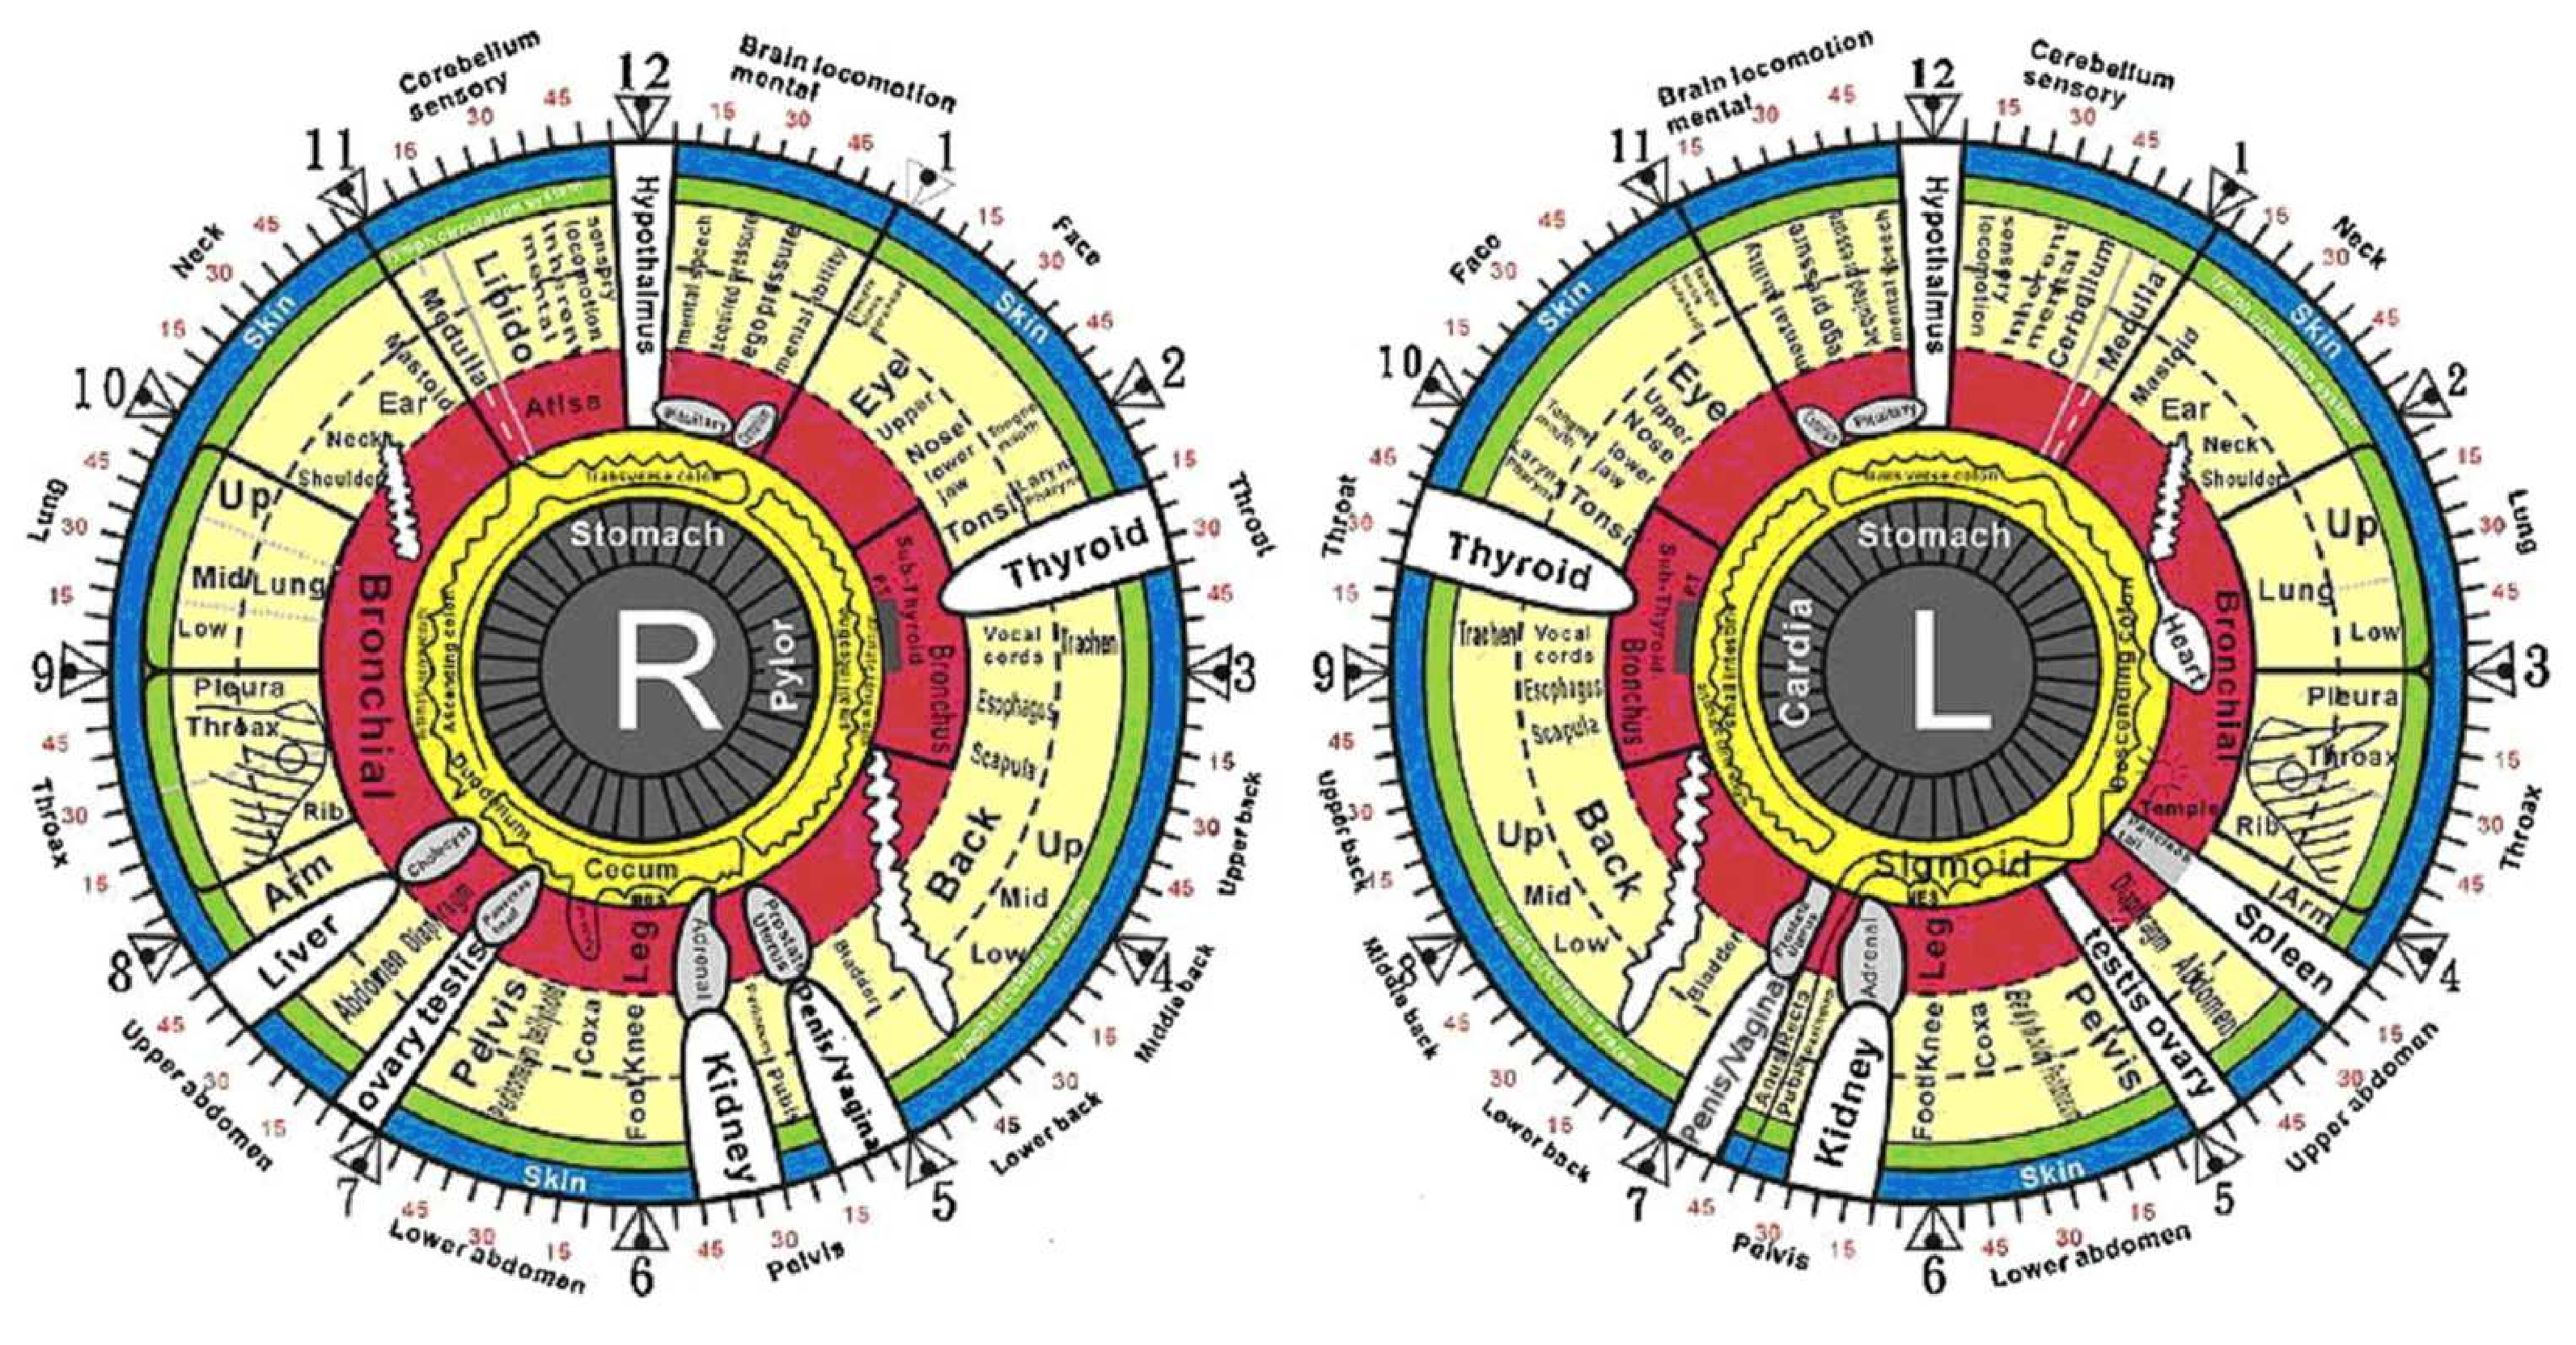
\includegraphics[width=0.68\textwidth]{imagens/mapa_iridologico_geral.png}
    \caption{Exemplo de mapa iridológico dos olhos direito (R) e esquerdo (L), mostrando a distribuição circular de áreas tradicionalmente associadas a órgãos e sistemas do corpo.}
    \label{fig:mapa-iridologico-geral}
\end{figure}

\subsection{Localização das regiões mencionadas no contexto do DM2}

Para o DM2, a literatura iridológica costuma destacar regiões associadas ao metabolismo e ao sistema digestivo, sobretudo ao \textbf{pâncreas}. Embora a Figura~\ref{fig:mapa-iridologico-geral} não rotule explicitamente o pâncreas, ela evidencia a lógica topográfica em que essa associação se insere: áreas digestivas (p.\ ex., \textit{Stomach}, \textit{Pylori}) aparecem em \textbf{zonas internas/intermediárias}, próximas à pupila, sugerindo que o pâncreas seria interpretado nessa vizinhança visceral. A leitura depende ainda da \textbf{posição angular} e é \textbf{bilateral} --- um mesmo órgão pode ocupar posições distintas nos olhos direito e esquerdo ---, o que exige cuidado ao definir regiões equivalentes entre amostras em estudos baseados em imagens.

\subsection{Relação com a análise regional e angular da íris}

A principal contribuição teórica desse tipo de mapa para o presente trabalho não está em validar clinicamente a iridologia, mas em fornecer uma referência histórica para a definição de regiões de interesse. A partir dessa lógica espacial, torna-se possível investigar computacionalmente:
\begin{itemize}
    \item se regiões internas associadas ao eixo digestivo/metabólico apresentam algum padrão discriminativo;
    \item se determinados setores angulares da íris concentram maior capacidade de diferenciação entre grupos;
    \item se tais padrões permanecem estáveis quando avaliados com controles metodológicos adequados.
\end{itemize}

Dessa forma, o mapa iridológico funciona aqui como uma \textbf{hipótese de localização}. Ele orienta onde observar possíveis sinais, mas não constitui, por si só, evidência de validade diagnóstica. Essa distinção é necessária porque estudos clínicos controlados e revisões críticas têm apontado que a iridologia, como método diagnóstico, não apresenta suporte robusto na literatura científica \citep{Simon1979JAMA, Knipschild1988BMJ, Ernst2000ArchOphthalmol}.

Em síntese, a Figura~\ref{fig:mapa-iridologico-geral} é útil para mostrar como a tradição iridológica organiza a íris em regiões e setores. No contexto do DM2, ela ajuda a justificar a escolha de análises locais e angulares, especialmente em áreas internas associadas ao eixo digestivo-metabólico. No entanto, essas associações devem ser interpretadas apenas como hipóteses exploratórias, a serem avaliadas de forma crítica e reprodutível.

% ====================== Trabalhos Relacionados ======================
\section{Trabalhos Relacionados}

A literatura recente especificamente dedicada a DM2 com imagens de íris permanece limitada em volume e heterogênea em delineamento metodológico. Para assegurar comparabilidade nesta seção, priorizam-se quatro estudos recentes (2022--2025) com foco explícito na classificação DM2 versus não-DM2 por aprendizado de máquina, assim como o artigo de referência deste trabalho.

\paragraph{Sruthi et al. (2022).}
No contexto da verificação computacional da hipótese iridológica para DM2, o estudo de \citet{SruthiEtAl2022IJPRAI} propõe uma estratégia orientada por região de interesse (ROI) associada ao pâncreas. Em contraste com abordagens de classificação global da íris, os autores privilegiam um recorte anatômico local, buscando maior sensibilidade a padrões texturais potencialmente discriminativos.

Do ponto de vista metodológico, são utilizadas imagens NIR de 178 voluntários, com segmentação da íris por FCN e extração subsequente da ROI pancreática para classificação. O artigo descreve o \textit{pipeline} de pré-processamento e treinamento em arquiteturas profundas; contudo, não foi identificado repositório público de código associado ao estudo.

No que se refere ao desempenho, foram comparadas as arquiteturas AlexNet, VGG-16 e ResNet-50. O melhor resultado foi reportado com AlexNet, alcançando acurácia de 95,85\%, sensibilidade de 95,80\% e especificidade de 95,85\%. Esses valores posicionam o estudo como uma referência recente de aprendizado profundo aplicado à classificação de DM2 por imagens de íris.

\paragraph{{\"O}nal et al. (2022).}
O trabalho de \citet{OnalEtAl2022MTA} reforça a linha de diagnóstico de DM2 por iridologia computacional. Sua contribuição central consiste em consolidar a aplicação de CNNs para inferência de DM2 a partir de imagens de íris em cenário experimental controlado.

No plano metodológico, os autores empregam arquitetura baseada em CNN para classificação binária e descrevem um fluxo de processamento direcionado ao suporte diagnóstico por imagens de íris. Assim como no trabalho anterior, não há indicação explícita de código-fonte público, tampouco descrição padronizada e completa da disponibilização dos dados.

Quanto ao desempenho, o estudo reporta acurácia de 94,12\% para a tarefa DM2 versus não-DM2, corroborando a competitividade da abordagem em relação a trabalhos contemporâneos. As métricas complementares (por exemplo, sensibilidade e especificidade por partição) não aparecem integralmente no material acessível.

\paragraph{Taghiyev et al. (2024).}
\citet{TaghiyevEtAl2024AICT} representa a transição para estudos mais recentes que exploram modelos de maior complexidade, com ênfase na estrutura relacional dos dados visuais. O trabalho é particularmente relevante por introduzir abordagem baseada em grafos em um domínio historicamente dominado por CNNs convencionais.

Metodologicamente, os autores combinam uma base pública e uma base local, realizando experimentos específicos com imagens do olho direito no subconjunto local. O modelo principal é uma GNN aplicada ao problema de detecção de DM2 por iridologia. De modo semelhante a outros estudos recentes, não foi identificado link de código aberto nem os dados.

No conjunto de resultados, o artigo reporta acurácia média de 92\% em 16 ensaios no subconjunto local mencionado. O valor indica desempenho competitivo; contudo, o estudo não apresenta métricas complementares como sensibilidade, especificidade e F1.

\paragraph{Anap et al. (2025).}
O estudo de \citet{AnapEtAl2025ICEC2NT} é um dos mais recentes no recorte de DM2 com imagens de íris e estrutura a análise a partir da comparação entre uma abordagem profunda (CNN) e uma abordagem clássica (SVM). Essa comparação direta é metodologicamente relevante para estimar o ganho incremental de arquiteturas profundas em relação a classificadores tradicionais.

No desenho metodológico, os autores utilizam imagens infravermelhas da íris e organizam o experimento para comparar ambos os classificadores no mesmo contexto de problema. O trabalho explicita o contraste entre os paradigmas de modelagem, mas não apresenta repositório público de código nem protocolo completo de disponibilização de dados para reprodução externa.

Nos resultados reportados, a CNN alcança acurácia de validação de 98,7\%, enquanto a SVM atinge 68,39\%, evidenciando diferença substancial entre os modelos na configuração analisada. Esse contraste reforça a tendência recente de superioridade de modelos profundos no domínio, ainda que a robustez externa dependa de validações adicionais.

\paragraph{Samant e Agarwal (2018).}
Como artigo de referência deste projeto, \citet{SamantAgarwal2018CMPB} formalizam a hipótese iridológica para DM2 em um \textit{pipeline} computacional de classificação a partir de imagens infravermelhas da íris. Metodologicamente, o estudo investiga 338 participantes (180 com DM2 e 158 controles), com captura simultânea de ambos os olhos, recorte de regiões de interesse associadas ao pâncreas segundo o mapa iridológico e extração de descritores estatísticos, de textura e de transformada wavelet discreta. Não foi identificado repositório público de código associado ao artigo. O trabalho também é relevante por tratar a informação regional de forma combinada, antecipando a discussão posterior deste relatório sobre a diferença entre avaliação setorial isolada e classificação multirregional concatenada.

Nos resultados reportados, o melhor desempenho foi obtido com \textit{Random Forest}, alcançando acurácia de 89,63\%, com especificidade de 0,9687 e sensibilidade de 0,988. Esse estudo permanece importante por traduzir alegações iridológicas em um protocolo computacional explícito, embora ainda dependa de validações adicionais de generalização e de controles metodológicos mais rígidos, como separação estrita por indivíduo e auditoria sistemática de robustez.

\begin{table}[htbp]
\centering
\caption{Trabalhos relacionados em ML para DM2 com imagens de íris.}
\label{tab:trabalhos-relacionados-dm2}
\small
\setlength{\tabcolsep}{5pt}
\setlength{\extrarowheight}{2pt}
\renewcommand{\arraystretch}{1.22}
\begin{tabularx}{\textwidth}{>{\raggedright\arraybackslash}p{0.14\textwidth} >{\centering\arraybackslash}p{0.07\textwidth} >{\raggedright\arraybackslash}X >{\raggedright\arraybackslash}p{0.16\textwidth} >{\raggedright\arraybackslash}X >{\centering\arraybackslash}p{0.12\textwidth}}
\toprule
\textbf{Referência} & \textbf{Ano} & \textbf{Features usadas} & \textbf{Classificador} & \textbf{Dataset} & \textbf{Acurácia} \\
\midrule
\citeauthor{SruthiEtAl2022IJPRAI} & 2022 & ROI pancreática em imagens NIR; \textit{features} aprendidas por DL após segmentação FCN & AlexNet, VGG-16, ResNet-50 & 178 voluntários (NIR) & 95,85\% \\
\addlinespace[2pt]

\citeauthor{OnalEtAl2022MTA} & 2022 & \textit{features} aprendidas por CNN em imagens de íris & CNN & Base de imagens de íris (detalhamento amostral não explicitado no resumo indexado) & 94,12\% \\
\addlinespace[2pt]

\citeauthor{TaghiyevEtAl2024AICT} & 2024 & Representações visuais modeladas em grafo (imagem de íris) & GNN & Base pública + base local (16 ensaios, olho direito na base local) & 92\% (média) \\
\addlinespace[2pt]

\citeauthor{AnapEtAl2025ICEC2NT} & 2025 & Padrões de textura em imagens infravermelhas da íris & CNN e SVM & Base de íris infravermelha (comparativo entre modelos) & 98,7\% (CNN); 68,39\% (SVM) \\
\addlinespace[2pt]

\citeauthor{SamantAgarwal2018CMPB} & 2018 & ROI pancreática em imagens IR; descritores estatísticos, de textura e de transformada wavelet discreta & RF (melhor resultado reportado) & 338 participantes (180 DM2, 158 controle), com captura simultânea de ambos os olhos & 89,63\% \\
\bottomrule
\end{tabularx}
\end{table}

\paragraph{Diferencial deste trabalho em relação aos anteriores.}
O diferencial central deste projeto é que o foco não está apenas em maximizar acurácia pontual, mas em \textbf{validar robustez e reprodutibilidade} com controles metodológicos explícitos. Diferentemente da maior parte dos estudos revisados, este relatório combina particionamento \textit{person-based} para reduzir vazamento por identidade, avaliação sistemática com múltiplas métricas clínicas (Acc, Sens, Esp, Prec e F1), testes de sensibilidade fotométrica e análises locais/radiais alinhadas às hipóteses iridológicas. Com isso, a principal contribuição deste trabalho é uma avaliação auditável e crítica da generalização do sinal, e não apenas a apresentação de um único valor alto de desempenho.

% ====================== Metodologia ======================
\section{Metodologia}

\subsection{Princípios do desenho experimental}
A metodologia deste projeto foi delineada para avaliar, de forma reprodutível e auditável, a hipótese de que imagens da íris possam conter \textbf{sinal estatístico} associado ao diabetes mellitus tipo 2 (DM2), isto é, que possam permitir alguma \textbf{separabilidade} entre grupos (DM2 vs.\ controle) quando avaliadas por métricas apropriadas. Em problemas de aprendizado de máquina com imagens biomédicas, desempenhos elevados podem decorrer de atalhos estatísticos, vazamento de identidade e artefatos de aquisição ou de pré-processamento. Para reduzir esses riscos e tornar as inferências mais robustas, o desenho experimental adota três princípios centrais:

\begin{enumerate}
    \item \textbf{Rastreabilidade:} cada etapa (dados, pré-processamento, extração de representações, parâmetros de treino e métricas) é registrada de modo que o experimento possa ser repetido, inspecionado e comparado.
    \item \textbf{Testes de sensibilidade:} o impacto de decisões de \textit{pipeline} (etapas e parametrizações) é avaliado de forma controlada, por meio de perturbações moderadas e comparação entre variantes (quando aplicável, incluindo versões com e sem determinadas perturbações) para identificar dependências críticas do desempenho.
    \item \textbf{Robustez e consistência:} um resultado é considerado relevante apenas se persistir sob variações controladas (por exemplo, sementes, estratégias de validação e perturbações moderadas).
\end{enumerate}

\subsection{Transformações fotométricas avaliadas}
\label{ref:transformacoes}
Para testar sensibilidade ao contraste/iluminação, são avaliadas transformações fotométricas padronizadas:
\begin{itemize}
    \item \textbf{Equalização global do histograma:} remapeia os níveis de intensidade com base na distribuição acumulada dos pixels, espalhando os tons por uma faixa mais ampla e aumentando o contraste global da imagem. Na prática, isso é útil quando a imagem está concentrada em uma faixa estreita de tons, embora possa não preservar tão bem diferenças locais muito sutis entre regiões distintas da íris. \citep{OpenCVHistEq}

    \item \textbf{CLAHE (\textit{Contrast Limited Adaptive Histogram Equalization}):} divide a imagem em pequenas regiões (\textit{tiles}) e aplica equalização de histograma em cada uma delas, o que aumenta o contraste local em vez de atuar apenas no contraste global. Em seguida, limita-se o crescimento excessivo dos picos do histograma (\textit{clip limit}) para evitar amplificação desproporcional de ruído, e as transições entre regiões são suavizadas por interpolação bilinear. Como exemplo concreto, pode-se considerar uma grade \(8\times 8\): se, em um \textit{tile} da íris, a maior parte dos pixels estiver concentrada entre intensidades 40 e 70, o CLAHE expande localmente essa faixa para tornar fibras, sulcos e variações de textura mais visíveis; ao mesmo tempo, o limite de contraste impede que poucos pixels muito claros dominem a transformação. Isso torna o método especialmente útil quando se deseja realçar detalhes locais da íris sem saturar regiões homogêneas. \citep{Zuiderveld1994CLAHE,OpenCVHistEq}

    \item \textbf{Desfoque gaussiano (\textit{Gaussian blur}):} convolui a imagem com um kernel gaussiano, suavizando componentes de alta frequência, como ruído, bordas finas e microdetalhes. Neste estudo, essa transformação funciona como um teste de robustez: se o desempenho cair de forma acentuada após a suavização, isso sugere dependência excessiva de microartefatos ou texturas muito finas do pré-processamento. \citep{OpenCVSmoothing}
\end{itemize}

Essas transformações são usadas como perturbações controladas para verificar estabilidade do desempenho sob variações plausíveis de aquisição e pré-processamento.

\subsection{Visão geral do pipeline}
O estudo segue um \textit{pipeline} fim-a-fim, estruturado para ser auditável e reprodutível. A lógica geral consiste em transformar imagens de íris em representações comparáveis e, em seguida, avaliar a consistência do desempenho na \textbf{separabilidade} entre grupos (DM2 vs.\ controle), sob controles de particionamento e reporte padronizado.

\begin{figure}[H]
    \centering
    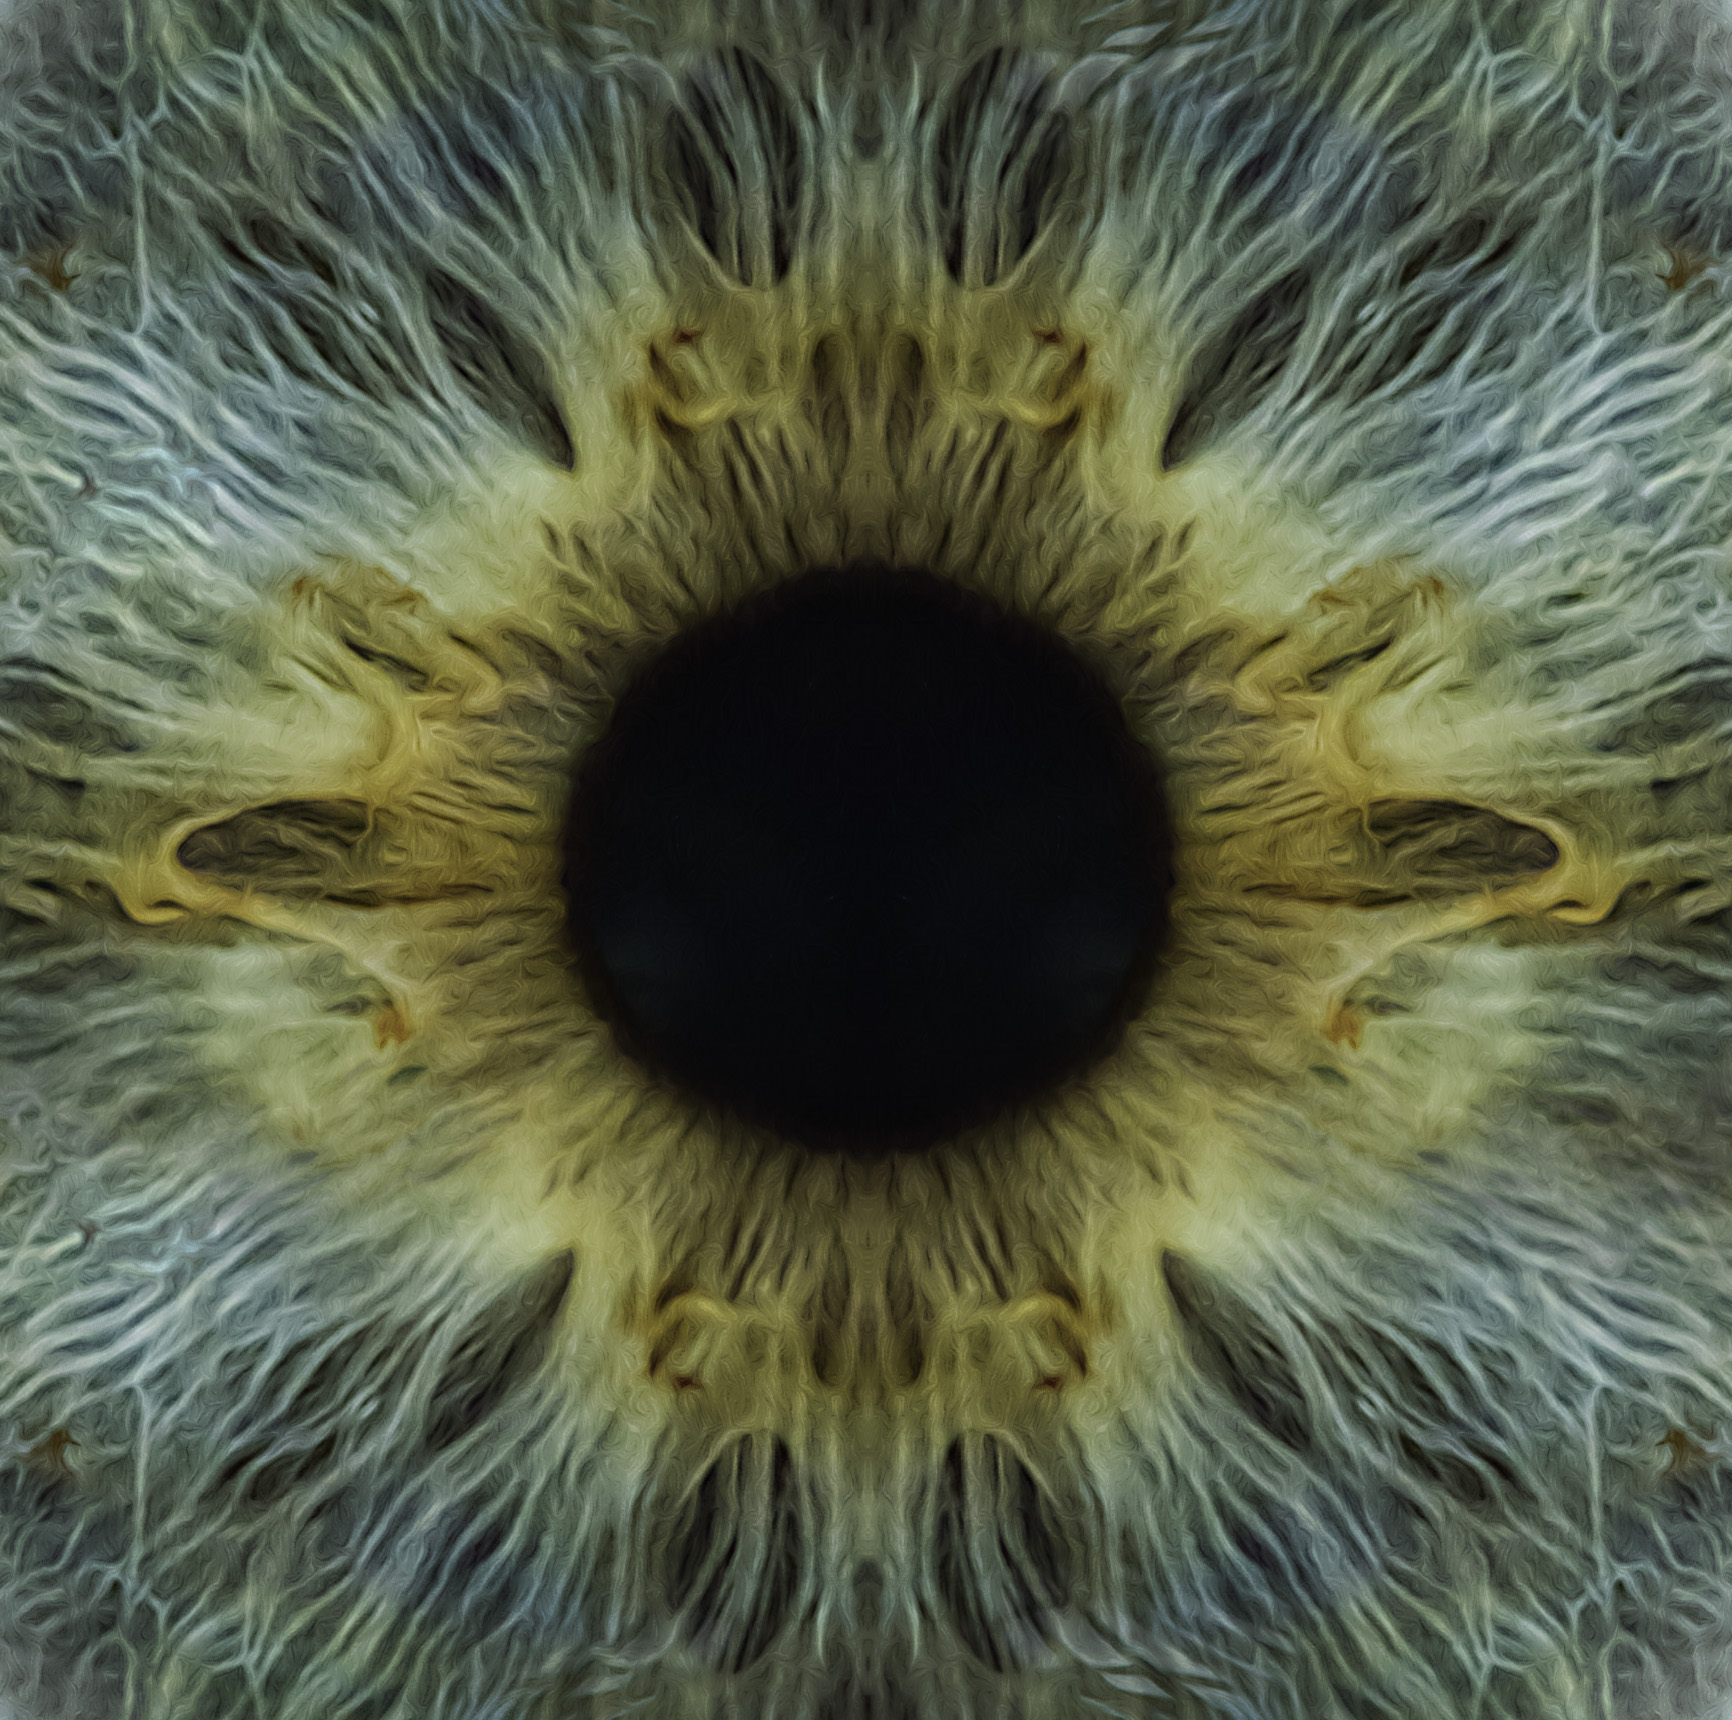
\includegraphics[width=0.30\textwidth]{iris_closeup.jpg}
    \caption{Exemplo ilustrativo de imagem de íris (macrofotografia), representando o tipo de entrada do \textit{pipeline}. A partir dessa aquisição, a íris é segmentada (isolando pupila, pálpebras e reflexos) e mapeada para uma representação canônica em coordenadas polares, de modo que as \textit{features} extraídas correspondam a regiões anatomicamente comparáveis entre indivíduos.}
    \label{fig:iris-original}
    {\footnotesize Fonte: Carlos Andrés Reyes / Wikimedia Commons (CC BY 2.0).}
\end{figure}

\begin{enumerate}
    \item \textbf{Coleta e organização dos dados.}
    As imagens são reunidas a partir do(s) conjunto(s) disponível(is) ao projeto. Nesta etapa, padronizam-se metadados essenciais: (i) rótulo clínico (DM2 / controle), (ii) lado do olho (esquerdo/direito), (iii) identidade do indivíduo (para controle de vazamento), e (iv) informações operacionais disponíveis (nome do arquivo, origem e parâmetros de captura). Metadados inconsistentes podem induzir particionamentos incorretos e aumentar o valor das métricas de forma espúria.

    \item \textbf{Pré-processamento inicial e controle fotométrico.}
    Realiza-se normalização básica de tamanho e intensidade para reduzir variações triviais de captura. Adicionalmente, aplicam-se as transformações fotométricas descritas na Seção~\ref{ref:transformacoes} (equalização global do histograma, CLAHE e desfoque gaussiano), com o objetivo de testar sensibilidade a contraste/iluminação.

    \item \textbf{Segmentação e delimitação anatômica.}
    Segmenta-se íris e pupila para isolar a região informativa e reduzir influência de regiões externas (pálpebra, reflexos e fundo). A segmentação também padroniza a área analisada, contribuindo para comparabilidade entre amostras.

    \item \textbf{Normalização geométrica (``rubber sheet'').}
    A íris segmentada é mapeada para uma representação canônica (coordenadas polares em uma grade retangular), facilitando comparações ponto-a-ponto mesmo na presença de variações de dilatação pupilar, rotação e enquadramento.

\item \textbf{Extração de representações (\textit{features}).}
São consideradas duas famílias de representações:
\begin{itemize}
    \item \textbf{\textit{Pixel features}:} vetor formado diretamente pelas intensidades dos pixels da íris após a normalização geométrica. Nessa representação, a informação é preservada em sua forma mais bruta, sem resumir previamente padrões locais ou relações espaciais, o que a torna uma linha de base (\textit{baseline}) útil para comparar o ganho real obtido com descritores mais elaborados. \citep{GonzalezWoods2018}

    \item \textbf{Descritores de textura/contraste:} medidas extraídas da íris normalizada, incluindo: (i) \textbf{estatísticas de intensidade e histogramas} (média, desvio padrão, assimetria e curtose), que descrevem a distribuição global dos níveis de cinza \citep{GonzalezWoods2018}; (ii) \textbf{\textit{Local Binary Patterns} (LBP)}, que codificam a microtextura comparando cada pixel à sua vizinhança, realçando bordas e sulcos \citep{Ojala2002LBP}; e (iii) \textbf{GLCM e descritores de Haralick} (contraste, correlação, energia e homogeneidade), que resumem a organização espacial da textura \citep{Haralick1973Texture}. Esses descritores são avaliados comparativamente para verificar se capturam padrões estruturais estáveis, e não apenas ruído ou artefatos do pré-processamento.
\end{itemize}

    \item \textbf{Treino e validação com controles.}
    Os modelos são treinados sob validação cruzada estratificada em \(K=5\) dobras (\textit{folds}), preservando a proporção de classes em cada divisão. Classificadores diversos (LR, SVM, RF, MLP e AdaBoost) são comparados para verificar consistência entre famílias de modelos; quando múltiplos modelos convergem, o resultado tende a ser mais estável.

    \item \textbf{Avaliação global e avaliação local.}
    A avaliação é conduzida em duas escalas:
    \begin{itemize}
        \item \textbf{Global (íris inteira):} mede desempenho geral utilizando a íris normalizada como um todo, sem impor hipótese espacial específica.
        \item \textbf{Local (por região):} aplica análises orientadas por mapeamentos iridológicos definidos na Seção~\ref{sec:locais}, verificando se o desempenho se concentra em regiões específicas de forma consistente.
    \end{itemize}

    \item \textbf{Testes de robustez e sensibilidade.}
    Por fim, são conduzidos testes para verificar dependência do desempenho em escolhas do \textit{pipeline}, incluindo perturbações controladas (fotometria, normalização e parâmetros de segmentação).
\end{enumerate}

\subsection{Particionamento e controle de vazamento (\textit{data leakage})}
Para reduzir risco de \textit{data leakage} e avaliar integridade do experimento, três esquemas de partição são empregados como controles complementares:

\begin{itemize}
    \item \textbf{L (Left Split):} utiliza apenas olhos esquerdos.
    \item \textbf{R (Right Split):} utiliza apenas olhos direitos.
    \item \textbf{Person-based:} separa por identidade, garantindo que nenhum indivíduo apareça simultaneamente em treino e teste. Este é o controle principal contra vazamento indireto de identidade e costuma ser o indicador mais informativo de generalização.
\end{itemize}

\subsection{Métricas}
A avaliação emprega métricas complementares, pois a acurácia isolada pode mascarar comportamentos relevantes. A partir de \(TP\), \(TN\), \(FP\) e \(FN\) (verdadeiros/falsos positivos e negativos), reportam-se: \textbf{acurácia} \(\left(\tfrac{TP+TN}{TP+TN+FP+FN}\right)\); \textbf{sensibilidade} (\textit{recall} da classe DM2, \(\tfrac{TP}{TP+FN}\)); \textbf{especificidade} \(\left(\tfrac{TN}{TN+FP}\right)\); \textbf{precisão} \(\left(\tfrac{TP}{TP+FP}\right)\); e \textbf{F1-score} (média harmônica entre precisão e sensibilidade, \(\tfrac{2TP}{2TP+FP+FN}\)). Quando cabível, cada métrica é reportada como média \(\pm\) desvio padrão entre os \(K\) \textit{folds} da validação cruzada, permitindo avaliar não apenas o desempenho médio, mas também sua estabilidade.
\subsection{Análises locais orientadas por mapeamentos iridológicos}
\label{sec:locais}
Os mapeamentos iridológicos considerados neste estudo são analisados por duas estratégias complementares:

\begin{itemize}
    \item \textbf{Setores angulares:} a íris normalizada é varrida por setores em passos de \SI{10}{\degree}, estimando desempenho por região. O objetivo é verificar se há concentração espacial consistente do efeito, em vez de flutuações aleatórias entre setores.

    \item \textbf{Região pancreática (malha espacial):} define-se uma região de interesse (ROI) associada ao pâncreas e subdivide-se essa região em uma malha \(\num{12}\times\num{12}\) células. Cada célula é avaliada para produzir mapas de calor e permitir comparação de estabilidade entre \textit{folds} e variações controladas do \textit{pipeline}.
\end{itemize}

% ====================== Configuração dos modelos e hiperparâmetros ======================
\subsection{Configuração dos modelos e hiperparâmetros}
\label{sec:hiperparametros}

Para assegurar \textbf{reprodutibilidade} e permitir auditoria independente dos resultados, esta seção detalha a configuração dos classificadores avaliados. Todos os modelos foram treinados sobre o mesmo conjunto de atributos (\textit{features} de pixel da íris normalizada), sob idêntico protocolo de particionamento \textit{person-based} e validação cruzada estratificada com \(K=5\) \textit{folds} e semente fixa (\texttt{random\_state}\,=\,42). Para os modelos sensíveis à escala das variáveis (Regressão Logística, SVM e MLP), aplicou-se padronização \textit{z-score} (\texttt{StandardScaler}) estimada \emph{exclusivamente} nas partições de treino de cada \textit{fold}, evitando qualquer vazamento de informação do conjunto de validação.

A Tabela~\ref{tab:hiperparametros-mlp} detalha a arquitetura e os hiperparâmetros do \textbf{Perceptron de Múltiplas Camadas (MLP)}, modelo que apresentou o melhor desempenho global entre os classificadores avaliados (cf.\ Tabela~\ref{tab:melhores-preliminares}). A topologia adotada --- duas camadas ocultas com 128 e 64 neurônios --- busca equilíbrio entre capacidade de representação e risco de sobreajuste, dada a elevada dimensionalidade das \textit{features} de pixel.

\begin{table}[H]
\centering
\caption{Arquitetura e hiperparâmetros do classificador MLP (modelo de melhor desempenho global).}
\label{tab:hiperparametros-mlp}
\small
\begin{tabularx}{\textwidth}{>{\raggedright\arraybackslash}p{6.4cm} >{\raggedright\arraybackslash}X}
\toprule
\textbf{Hiperparâmetro / Componente} & \textbf{Valor / Configuração} \\
\midrule
Arquitetura (camadas ocultas) & 2 camadas totalmente conectadas \\
Neurônios por camada oculta & 128 e 64 \\
Função de ativação (camadas ocultas) & ReLU (\textit{Rectified Linear Unit}) \\
Camada de saída & 2 neurônios com \textit{softmax} (classificação binária: DM2 vs.\ controle) \\
Otimizador (\textit{solver}) & Adam (\(\beta_1=0{,}9\); \(\beta_2=0{,}999\)) \\
Taxa de aprendizado inicial & \(10^{-3}\) (constante) \\
Regularização L2 (\(\alpha\)) & \(10^{-4}\) \\
Tamanho do \textit{batch} & 32 \\
Número máximo de épocas & 300 \\
Parada antecipada (\textit{early stopping}) & Sim (10\% de validação interna; paciência de 10 épocas) \\
Padronização das entradas & \textit{z-score} (\texttt{StandardScaler}) \\
Semente aleatória (\texttt{random\_state}) & 42 \\
\bottomrule
\end{tabularx}
\end{table}

Para os demais classificadores, a Tabela~\ref{tab:hiperparametros-gerais} resume as principais configurações adotadas. Sempre que aplicável, mantiveram-se valores padrão consolidados na literatura e na implementação de referência (\textit{scikit-learn}), de modo a priorizar a \textbf{comparabilidade} entre modelos e a transparência do protocolo.

\begin{table}[H]
\centering
\caption{Principais hiperparâmetros dos demais classificadores avaliados.}
\label{tab:hiperparametros-gerais}
\small
\begin{tabularx}{\textwidth}{>{\raggedright\arraybackslash}p{3.4cm} >{\raggedright\arraybackslash}X}
\toprule
\textbf{Modelo} & \textbf{Principais hiperparâmetros} \\
\midrule
Regressão Logística & Penalidade L2; \(C=1{,}0\); \textit{solver} \texttt{lbfgs}; máx.\ de iterações 1000; \texttt{class\_weight}\,=\,\textit{balanced} \\
SVM (\textit{kernel} RBF) & \textit{Kernel} RBF; \(C=1{,}0\); \(\gamma=\)\,\textit{scale}; estimativa de probabilidade habilitada \\
Random Forest & 300 árvores; critério de \textit{Gini}; profundidade máxima livre; \texttt{max\_features}\(=\sqrt{n}\); \textit{bootstrap} ativo \\
AdaBoost & Estimador base: árvore de decisão (\textit{stump}, profundidade 1); 200 estimadores; taxa de aprendizado \(1{,}0\); algoritmo SAMME.R \\
Protocolo comum & Validação cruzada estratificada \textit{person-based} (\(K=5\)); semente 42; padronização \textit{z-score} para LR, SVM e MLP \\
\bottomrule
\end{tabularx}
\end{table}

% ====================== Resultados ======================
\section{Resultados da avaliação Global}

\subsection{Panorama geral dos resultados}
Os resultados indicam um padrão consistente: ao adotar particionamento \textit{person-based} (isto é, sem compartilhamento de indivíduos entre treino e teste), observa-se aumento substancial de desempenho. Nesta seção, reportam-se inicialmente resultados com \emph{pixel features} como \textbf{baseline} (representação direta, de menor complexidade), pois estabelece uma referência clara para interpretar ganhos (ou regressões) quando se introduzem descritores mais elaborados e transformações fotométricas.

A Tabela~\ref{tab:feat-metrics-dataset-classifier} detalha os valores completos por \textit{dataset}, classificador e métrica, e a Figura~\ref{fig:acc-datasets} sintetiza esse comportamento de forma sistemática.

\begin{table}[htbp]
\centering
\caption{Desempenho por \textit{dataset} e classificador utilizando \emph{pixel features}. Cada linha reporta uma métrica (Acc, Sens, Esp, Prec, F1).}
\label{tab:feat-metrics-dataset-classifier}
\small
\setlength{\tabcolsep}{4pt}
\renewcommand{\arraystretch}{1.08}
\begin{tabular}{llccccc}
\toprule
\textbf{Dataset} & \textbf{Métrica} & \textbf{AdaBoost} & \textbf{MLP} & \textbf{RF} & \textbf{SVM} & \textbf{LR} \\
\midrule
\texttt{L\_split} & Acc  & 0.6312 & 0.6745 & 0.6138 & 0.7285 & 0.6742 \\
                 & Sens & 0.6270 & 0.6700 & 0.6080 & 0.7240 & 0.6690 \\
                 & Esp  & 0.6360 & 0.6790 & 0.6200 & 0.7330 & 0.6800 \\
                 & Prec & 0.6340 & 0.6770 & 0.6160 & 0.7310 & 0.6760 \\
                 & F1   & 0.6300 & 0.6730 & 0.6120 & 0.7270 & 0.6720 \\
\addlinespace[5pt]
\texttt{R\_split} & Acc  & 0.7282 & 0.7229 & 0.6176 & 0.7542 & 0.7784 \\
                 & Sens & 0.7240 & 0.7190 & 0.6120 & 0.7500 & 0.7740 \\
                 & Esp  & 0.7330 & 0.7270 & 0.6240 & 0.7590 & 0.7830 \\
                 & Prec & 0.7310 & 0.7250 & 0.6200 & 0.7570 & 0.7810 \\
                 & F1   & 0.7270 & 0.7220 & 0.6160 & 0.7530 & 0.7770 \\
\addlinespace[5pt]
\texttt{personBase} & Acc  & 0.8779 & \textbf{0.9236} & 0.8367 & 0.8824 & 0.9081 \\
                   & Sens & 0.8720 & \textbf{0.9260} & 0.8310 & 0.8780 & 0.9040 \\
                   & Esp  & 0.8840 & \textbf{0.9210} & 0.8420 & 0.8870 & 0.9120 \\
                   & Prec & 0.8810 & \textbf{0.9280} & 0.8390 & 0.8860 & 0.9120 \\
                   & F1   & 0.8760 & \textbf{0.9270} & 0.8350 & 0.8820 & 0.9080 \\
\bottomrule
\end{tabular}
\end{table}

\begin{figure}[H]
\centering
\begin{tikzpicture}
\begin{axis}[
    ybar,
    bar width=7pt,
    width=0.9\textwidth,
    height=5.0cm,
    enlarge x limits=0.15,
    ymin=0.55, ymax=1.0,
    ylabel={Acur\'acia},
    symbolic x coords={AdaBoost,MLP,RF,SVM,LR},
    xtick=data,
    tick label style={font=\footnotesize},
    label style={font=\small},
    ymajorgrids, grid style={gray!20},
    legend style={at={(0.5,-0.16)}, anchor=north, legend columns=3, font=\footnotesize, draw=gray!40},
]
\addplot[fill=blue!25, draw=blue!55!black] coordinates {(AdaBoost,0.6312)(MLP,0.6745)(RF,0.6138)(SVM,0.7285)(LR,0.6742)};
\addplot[fill=orange!35, draw=orange!75!black] coordinates {(AdaBoost,0.7282)(MLP,0.7229)(RF,0.6176)(SVM,0.7542)(LR,0.7784)};
\addplot[fill=teal!35, draw=teal!70!black] coordinates {(AdaBoost,0.8779)(MLP,0.9236)(RF,0.8367)(SVM,0.8824)(LR,0.9081)};
\legend{\texttt{L\_split}, \texttt{R\_split}, \texttt{personBase}}
\end{axis}
\end{tikzpicture}
\caption{Acur\'acia por classificador em cada esquema de particionamento (\textit{pixel features}). O ganho consistente do cen\'ario \texttt{personBase} sobre \texttt{L\_split}/\texttt{R\_split} evidencia que, ao controlar o vazamento por indiv\'iduo, o desempenho cresce de forma homog\^enea entre modelos --- com pico do MLP ($0{,}9236$). As m\'etricas Sens/Esp/Prec/F1 acompanham de perto a acur\'acia.}
\label{fig:acc-datasets}
{\footnotesize Fonte: Elaborado pelo autor (2026).}
\end{figure}

No cenário \texttt{personBase}, registram-se os maiores valores para todos os classificadores avaliados, com destaque para:
\begin{itemize}
    \item \textbf{\texttt{personBase + MLP}:} Acc \(\approx 0{,}9236\) (com Sens/Esp/Prec/F1 igualmente elevados), configurando o melhor desempenho observado nesta etapa;
    \item \textbf{\texttt{personBase + LR}:} Acc \(\approx 0{,}9081\), indicando que um modelo linear também retém capacidade discriminativa relevante;
    \item \textbf{\texttt{personBase + SVM}:} Acc \(\approx 0{,}8824\), corroborando o padrão ao se utilizar um classificador distinto.
\end{itemize}

Esse comportamento é informativo porque o particionamento \texttt{personBase} reduz uma via recorrente de \textit{data leakage} em imagens biomédicas: a exploração indireta de características idiossincráticas do indivíduo. Assim, o desempenho elevado sob esse controle é compatível com um cenário em que os modelos dependem menos de reconhecimento de identidade e mais de informação associada ao rótulo clínico, ainda que essa interpretação permaneça condicionada às análises de robustez e aos controles metodológicos descritos nas seções anteriores.

% ------------------------------------------------------------------

\subsection{Síntese das melhores configurações (global e com transformações)}
Para facilitar a leitura, a Tabela~\ref{tab:melhores-preliminares} consolida os melhores desempenhos observados no estudo, distinguindo (i) a melhor execução com \textit{pixel features}, como visto na subseção anterior, e (ii) a melhor execução ao empregar transformações fotométricas. Reporta-se ainda o modelo LR (modelo de referência), por ser um \textit{baseline} competitivo e mais interpretável, útil como comparação quando modelos mais complexos apresentam variações. Por fim, apresenta-se o \textbf{ganho relativo médio} observado com CLAHE.

\begin{table}[htbp]
\centering
\caption{Principais resultados (melhores configurações observadas no estudo).}
\label{tab:melhores-preliminares}
\small
\setlength{\tabcolsep}{4pt}
\renewcommand{\arraystretch}{1.15}

\begin{tabular}{@{}p{0.34\textwidth} p{0.18\textwidth} p{0.22\textwidth} r@{}}
\toprule
\textbf{Cenário} & \textbf{Dataset} & \textbf{Configuração} & \textbf{Valor} \\
\midrule
\multirow{5}{*}{Melhor global (\textit{pixel features})} & \multirow{5}{*}{\texttt{personBase}} & \multirow{5}{*}{MLP} & Acc = 0,9236 \\
& & & Sens = 0,926 \\
& & & Esp = 0,921 \\
& & & Prec = 0,928 \\
& & & F1 = 0,927 \\
\addlinespace[6pt]

\multirow{5}{*}{Melhor com transf.\ fotométrica} & \multirow{5}{*}{\texttt{personBase}} & \multirow{5}{*}{MLP + Histogram} & Acc = 0,9233 \\
& & & Sens = 0,925 \\
& & & Esp = 0,922 \\
& & & Prec = 0,927 \\
& & & F1 = 0,926 \\
\addlinespace[6pt]

\multirow{5}{*}{Modelo alternativo (referência)} & \multirow{5}{*}{\texttt{personBase}} & \multirow{5}{*}{LR} & Acc = 0,9081 \\
& & & Sens = 0,904 \\
& & & Esp = 0,912 \\
& & & Prec = 0,912 \\
& & & F1 = 0,908 \\
\addlinespace[6pt]

\multirow{5}{*}{Ganho relativo médio CLAHE} & \multirow{5}{*}{\texttt{personBase}} & \multirow{5}{*}{CLAHE (média)} & Acc = +1,09\% \\
& & & Sens = +1,1\% \\
& & & Esp = +1,0\% \\
& & & Prec = +1,1\% \\
& & & F1 = +1,1\% \\
\bottomrule
\end{tabular}
\end{table}

Na tabela, a linha \textbf{Ganho relativo médio com CLAHE} resume apenas resultados obtidos no cenário \texttt{personBase}, por ser a configuração metodologicamente mais adequada neste estudo. Para cada configuração avaliada dentro do \texttt{personBase}, calcula-se o ganho relativo entre a versão com CLAHE e a versão original, segundo
\[
\Delta(\%) = 100 \cdot \frac{m_{\text{CLAHE}} - m_{\text{original}}}{m_{\text{original}}},
\]
em que \(m\) representa a métrica analisada (por exemplo, acurácia, sensibilidade ou F1). O valor reportado na tabela corresponde, então, à média desses ganhos relativos entre as diferentes combinações avaliadas (por exemplo, modelos, representações e variações de pré-processamento) dentro do \texttt{personBase}.

Assim, \textbf{Acc = +1{,}09\%} significa que, em média, a acurácia com CLAHE foi \(1{,}09\%\) maior do que a acurácia da versão sem CLAHE, considerando sempre comparações entre a mesma configuração antes e depois da transformação. Por exemplo, se uma configuração tivesse acurácia original de \(0{,}9000\), um ganho relativo de \(+1{,}09\%\) corresponderia a \(0{,}9000 \times 1{,}0109 = 0{,}9098\), isto é, um ganho absoluto de aproximadamente \(0{,}0098\) (ou \(0{,}98\) ponto percentual).

O CLAHE é incluído não por se assumir, a priori, superioridade absoluta, mas por aumentar o contraste local e reduzir a dependência de variações de iluminação --- particularmente relevante em imagens de íris. Cabe distinguir \textbf{melhor resultado isolado} de \textbf{efeito médio}: o melhor desempenho individual permanece o MLP com \textit{pixel features} em \texttt{personBase} (\(Acc = 0{,}9236\)), com a melhor execução fotométrica (MLP + Histogram) muito próxima (\(0{,}9233\)); ainda assim, o CLAHE tende a melhorar o desempenho de forma consistente na média, configurando-se como estratégia promissora de robustez.

% ------------------------------------------------------------------

\subsection{Estabilidade e consistência dos resultados}

A interpretação de acurácias elevadas requer, além do valor médio obtido, a análise da variabilidade entre partições de validação. Um desempenho alto pode decorrer de flutuações amostrais em uma partição específica ou de efeitos metodológicos não totalmente controlados. Por essa razão, o desvio padrão por \textit{fold} é empregado como medida complementar de consistência, pois permite avaliar se o desempenho permanece relativamente estável sob diferentes reamostragens da validação cruzada.

Para reprodutibilidade, adotou-se semente aleatória fixa (\texttt{42}) na geração das partições e nas rotinas estocásticas dos classificadores; reavaliações com múltiplas sementes são previstas como trabalho futuro.

A Tabela~\ref{tab:feat-top4} apresenta as combinações de maior desempenho no \textbf{baseline com \emph{pixel features}}, isto é, na configuração sem transformações fotométricas. Assim, esta tabela considera apenas pares \textit{dataset + classificador}, comparando diretamente diferentes algoritmos de classificação (por exemplo, MLP, LR, SVM e AdaBoost) sobre a mesma representação-base. Transformações fotométricas isoladas ou compostas --- como \textit{Histogram}, CLAHE, \textit{Gaussian blur} ou combinações do tipo \textit{Histogram + CLAHE + blur} --- não são incluídas nesta tabela, pois são analisadas separadamente nas subseções dedicadas aos experimentos com pré-processamento.

Nesta tabela, a acurácia é reportada em porcentagem, enquanto o desvio padrão é expresso em pontos percentuais (pp), para manter comparabilidade direta. Assim, por exemplo, uma acurácia de \(0{,}9236\) corresponde a \(92{,}36\%\).

\begin{table}[htbp]
\centering
\caption{Top 4 combinações (\textit{dataset} + classificador) por acurácia no baseline com \emph{pixel features}, sem transformações fotométricas.}
\label{tab:feat-top4}
\scriptsize
\setlength{\tabcolsep}{3pt}
\renewcommand{\arraystretch}{1.12}
\begin{tabular}{cllcccccc}
\toprule
\textbf{Pos.} & \textbf{Dataset} & \textbf{Classif.} & \textbf{Acc (\%)} & \textbf{Sens (\%)} & \textbf{Esp (\%)} & \textbf{Prec (\%)} & \textbf{F1 (\%)} & \textbf{DP (pp)} \\
\midrule
1 & \texttt{personBase} & MLP      & 92,36 & 92,60 & 92,10 & 92,80 & 92,70 & 3,59 \\
2 & \texttt{personBase} & LR       & 90,81 & 90,40 & 91,20 & 91,20 & 90,80 & 3,50 \\
3 & \texttt{personBase} & SVM      & 88,24 & 87,80 & 88,70 & 88,60 & 88,20 & 6,22 \\
4 & \texttt{personBase} & AdaBoost & 87,79 & 87,20 & 88,40 & 88,10 & 87,60 & 5,07 \\
\bottomrule
\end{tabular}
\end{table}

Os resultados indicam que o \texttt{personBase} sustenta desempenho elevado em diferentes famílias de classificadores, e não apenas em um único algoritmo. Esse comportamento reforça a interpretação de que o efeito observado está associado, em alguma medida, ao particionamento e à representação adotada, e não exclusivamente a uma escolha específica de modelo. Em particular, o melhor resultado da tabela é obtido com MLP no \texttt{personBase}, com \(92{,}36\%\) de acurácia (equivalente a \(0{,}9236\)), enquanto LR, SVM e AdaBoost também mantêm desempenho competitivo no mesmo cenário. Isso é desejável em análises de reprodutibilidade, pois sugere consistência do efeito em mais de uma família de classificadores.

Quanto à dispersão entre \textit{folds}, os desvios de \(3{,}59\) pp (MLP) e \(3{,}50\) pp (LR) indicam boa estabilidade, ao passo que \(6{,}22\) pp (SVM) e \(5{,}07\) pp (AdaBoost) revelam maior sensibilidade à composição das partições. Assim, embora todas as combinações apresentem acurácias competitivas, MLP e LR destacam-se pela maior consistência entre as reamostragens.

% ------------------------------------------------------------------

\subsection{Efeito de transformações fotométricas na robustez}
A comparação entre dados originais e versões recriadas por transformações fotométricas fornece um teste inicial de sensibilidade do \textit{pipeline} a variações de contraste, distribuição de intensidades e suavização (por exemplo, diferenças de iluminação/exposição entre capturas, alterações no contraste local e pequenas variações de nitidez). Para evitar ambiguidades de interpretação, a Figura~\ref{fig:robustez} fixa o mesmo classificador em todas as comparações, utilizando o \textbf{MLP} sobre a mesma representação-base com \textit{pixel features}. Dessa forma, cada grupo de barras mostra o efeito da transformação fotométrica sobre uma mesma configuração de referência.

Além das transformações isoladas (\textit{Histogram}, CLAHE e \textit{Blur}), inclui-se uma configuração composta (\textit{Histogram + CLAHE + Blur}), para verificar se a combinação sequencial de ajustes produz ganho adicional ou introduz degradação por excesso de pré-processamento.

\begin{figure}[H]
\centering
\begin{tikzpicture}
\begin{axis}[
    ybar, bar width=6pt,
    width=0.9\textwidth, height=5.0cm,
    enlarge x limits=0.14,
    ymin=0.6, ymax=1.0,
    ylabel={Acur\'acia},
    symbolic x coords={Original,Histogram,CLAHE,Blur,Composta},
    xtick=data,
    xticklabel style={font=\footnotesize},
    tick label style={font=\footnotesize}, label style={font=\small},
    ymajorgrids, grid style={gray!20},
    legend style={at={(0.5,-0.18)}, anchor=north, legend columns=3, font=\footnotesize, draw=gray!40},
]
\addplot[fill=blue!25, draw=blue!55!black] coordinates {(Original,0.7121)(Histogram,0.7303)(CLAHE,0.7243)(Blur,0.6982)(Composta,0.7148)};
\addplot[fill=orange!35, draw=orange!75!black] coordinates {(Original,0.7781)(Histogram,0.7493)(CLAHE,0.8009)(Blur,0.7637)(Composta,0.7931)};
\addplot[fill=teal!35, draw=teal!70!black] coordinates {(Original,0.9236)(Histogram,0.9233)(CLAHE,0.9218)(Blur,0.9174)(Composta,0.9196)};
\legend{\texttt{L\_split}, \texttt{R\_split}, \texttt{personBase}}
\end{axis}
\end{tikzpicture}
\caption{Robustez a transforma\c{c}\~oes fotom\'etricas (classificador MLP fixo, \textit{pixel features}). O cen\'ario \texttt{personBase} mant\'em acur\'acia alta e praticamente est\'avel ($\approx 0{,}92$) sob todas as transforma\c{c}\~oes, evidenciando robustez; em \texttt{L\_split}/\texttt{R\_split} o efeito depende do particionamento. As demais m\'etricas (Sens/Esp/Prec/F1) acompanham a acur\'acia.}
\label{fig:robustez}
{\footnotesize Fonte: Elaborado pelo autor (2026).}
\end{figure}

A Tabela~\ref{tab:original-vs-recriado} apresenta os valores numéricos completos por partição e métrica, complementando a leitura gráfica da Figura~\ref{fig:robustez}. Nessa formulação, o valor \(0{,}9236\) das tabelas anteriores reaparece naturalmente como \(92{,}36\%\) na linha de \texttt{personBase} e coluna \textbf{Original}, pois trata-se da mesma configuração de referência (MLP com \textit{pixel features}), apenas expressa aqui em porcentagem.

\begin{table}[htbp]
\centering
\caption{Comparação entre dados originais e versões recriadas por transformações fotométricas, mantendo fixos o classificador (MLP) e a representação-base (\emph{pixel features}). A coluna composta representa uma aplicação sequencial de \emph{Histogram + CLAHE + Blur}.}
\label{tab:original-vs-recriado}
\scriptsize
\setlength{\tabcolsep}{3pt}
\renewcommand{\arraystretch}{1.10}
\begin{tabular}{llccccc}
\toprule
\textbf{Dataset} & \textbf{Métrica} & \textbf{Original} & \textbf{Histogram} & \textbf{CLAHE} & \textbf{Blur} & \textbf{Hist.+CLAHE+Blur} \\
\midrule
\texttt{L\_split} & Acc  & 71.21\% & 73.03\% & 72.43\% & 69.82\% & 71.48\% \\
                  & Sens & 0.705   & 0.723   & 0.715   & 0.690   & 0.709 \\
                  & Esp  & 0.719   & 0.736   & 0.732   & 0.708   & 0.717 \\
                  & Prec & 0.714   & 0.731   & 0.727   & 0.698   & 0.711 \\
                  & F1   & 0.709   & 0.728   & 0.721   & 0.693   & 0.710 \\
\addlinespace[2pt]

\texttt{R\_split} & Acc  & 77.81\% & 74.93\% & 80.09\% & 76.37\% & 79.31\% \\
                  & Sens & 0.774   & 0.749   & 0.796   & 0.759   & 0.786 \\
                  & Esp  & 0.784   & 0.756   & 0.806   & 0.771   & 0.801 \\
                  & Prec & 0.781   & 0.751   & 0.804   & 0.767   & 0.795 \\
                  & F1   & 0.778   & 0.746   & 0.800   & 0.763   & 0.790 \\
\addlinespace[2pt]

\texttt{personBase} & Acc  & 92.36\% & 92.33\% & 92.18\% & 91.74\% & 91.96\% \\
                    & Sens & 0.926   & 0.925   & 0.923   & 0.919   & 0.921 \\
                    & Esp  & 0.921   & 0.922   & 0.920   & 0.915   & 0.918 \\
                    & Prec & 0.928   & 0.927   & 0.925   & 0.921   & 0.923 \\
                    & F1   & 0.927   & 0.926   & 0.924   & 0.920   & 0.922 \\
\bottomrule
\end{tabular}
\end{table}

Em termos interpretativos, essa organização permite distinguir com maior clareza três níveis de análise: (i) o desempenho da configuração original de referência, (ii) o efeito de cada transformação fotométrica aplicada isoladamente e (iii) o efeito de uma composição representativa de transformações. Os resultados sugerem que o impacto do pré-processamento depende do particionamento considerado: em \texttt{L\_split}, a equalização de histograma apresenta o melhor ganho; em \texttt{R\_split}, o CLAHE mostra o efeito mais favorável; já em \texttt{personBase}, a configuração original com \textit{pixel features} permanece como melhor resultado observado, com desempenho muito próximo ao caso com \textit{Histogram}.

Assim, com base nessa análise, não se conclui que uma transformação fotométrica seja universalmente superior ao caso original. Em vez disso, observa-se que algumas transformações podem melhorar o desempenho em cenários específicos, enquanto em outros a configuração base permanece mais forte. Isso é consistente com a interpretação de que as transformações fotométricas atuam como teste de robustez: elas ajudam a revelar a sensibilidade do \textit{pipeline} a variações de contraste e iluminação, sem necessariamente substituir o \textit{baseline} como melhor escolha em todos os contextos.

\section{Resultados da avaliação Local}
Esta seção reúne os resultados exploratórios de avaliação local, isto é, análises focadas em regiões específicas da íris em vez de apenas no desempenho global do \textit{pipeline}. O objetivo aqui é verificar se existem áreas com concentração espacial de sinal discriminativo, o que pode ser descrito tanto em coordenadas locais (grade \(12\times 12\)) quanto em coordenadas angulares (varredura setorial associada à chamada Cruz de Andréas).

\subsection{Análise micro-regional da região pancreática (grade \texorpdfstring{$12\times 12$}{12x12})}
\noindent\textit{Configuração experimental:} classificador \textbf{Regressão Logística (LR)}, representação \emph{pixel features}, transformação fotométrica \textbf{Equalização de Histograma}, particionamento \texttt{personBase}.

Para aprofundar a investigação local, foi definida uma região de interesse (ROI) associada ao pâncreas e subdividida em uma malha espacial \(12\times 12\). Essa decomposição permite avaliar o desempenho do classificador em células locais da ROI, verificando se há concentração espacial de desempenho elevado em áreas pequenas e contíguas --- compatível com um sinal local focal. A grade é indexada por linha e coluna (\(0\) a \(11\)), com a célula \((0,0)\) no canto superior esquerdo.

A Tabela~\ref{tab:pancreas-grid-indexado} apresenta a distribuição espacial das acurácias locais na ROI pancreática, com indexação explícita das linhas e colunas da grade. Os valores correspondem à acurácia obtida em cada célula da malha, permitindo visualizar a concentração espacial dos maiores desempenhos em uma vizinhança específica da região analisada.

\begin{table}[htbp]
\centering
\caption{Mapa de acurácia local na ROI pancreática com indexação explícita das linhas e colunas da grade \(12\times 12\). A célula \((0,0)\) está no canto superior esquerdo.}
\label{tab:pancreas-grid-indexado}
\scriptsize
\setlength{\tabcolsep}{3.8pt}
\renewcommand{\arraystretch}{1.1}
\begin{tabular}{c|cccccccccccc}
\toprule
\textbf{Linha/Col.} & \textbf{0} & \textbf{1} & \textbf{2} & \textbf{3} & \textbf{4} & \textbf{5} & \textbf{6} & \textbf{7} & \textbf{8} & \textbf{9} & \textbf{10} & \textbf{11} \\
\midrule
\textbf{0}  & 0.61 & 0.62 & 0.60 & 0.58 & 0.59 & 0.61 & 0.63 & 0.60 & 0.58 & 0.59 & 0.60 & 0.61 \\
\textbf{1}  & 0.62 & 0.65 & 0.68 & 0.64 & 0.62 & 0.65 & 0.67 & 0.62 & 0.60 & 0.61 & 0.62 & 0.63 \\
\textbf{2}  & 0.60 & 0.68 & 0.88 & 0.91 & 0.89 & 0.70 & 0.65 & 0.61 & 0.59 & 0.60 & 0.61 & 0.60 \\
\textbf{3}  & 0.59 & 0.66 & 0.92 & 0.95 & 0.90 & 0.72 & 0.64 & 0.60 & 0.58 & 0.59 & 0.60 & 0.62 \\
\textbf{4}  & 0.61 & 0.64 & 0.87 & 0.89 & 0.86 & 0.69 & 0.63 & 0.62 & 0.60 & 0.61 & 0.63 & 0.61 \\
\textbf{5}  & 0.63 & 0.62 & 0.65 & 0.67 & 0.64 & 0.62 & 0.61 & 0.64 & 0.62 & 0.63 & 0.61 & 0.60 \\
\textbf{6}  & 0.60 & 0.61 & 0.63 & 0.65 & 0.62 & 0.60 & 0.59 & 0.61 & 0.63 & 0.60 & 0.59 & 0.58 \\
\textbf{7}  & 0.58 & 0.60 & 0.61 & 0.62 & 0.60 & 0.59 & 0.58 & 0.60 & 0.61 & 0.62 & 0.60 & 0.59 \\
\textbf{8}  & 0.59 & 0.59 & 0.60 & 0.61 & 0.59 & 0.58 & 0.57 & 0.59 & 0.60 & 0.61 & 0.59 & 0.58 \\
\textbf{9}  & 0.60 & 0.61 & 0.62 & 0.60 & 0.58 & 0.59 & 0.60 & 0.62 & 0.63 & 0.60 & 0.58 & 0.59 \\
\textbf{10} & 0.61 & 0.62 & 0.61 & 0.59 & 0.60 & 0.61 & 0.62 & 0.61 & 0.62 & 0.61 & 0.60 & 0.60 \\
\textbf{11} & 0.58 & 0.60 & 0.59 & 0.58 & 0.59 & 0.60 & 0.61 & 0.59 & 0.58 & 0.59 & 0.60 & 0.61 \\
\bottomrule
\end{tabular}
\end{table}

A Figura~\ref{fig:pancreas-grid} apresenta a mesma informação da Tabela~\ref{tab:pancreas-grid-indexado} em um formato visual de mapa de calor, facilitando a identificação do agrupamento de células de alto desempenho na ROI pancreática.

\begin{figure}[H]
\centering
\begin{tikzpicture}
\begin{axis}[
    width=0.56\textwidth, height=0.56\textwidth,
    enlargelimits=false, axis on top,
    xlabel={Coluna}, ylabel={Linha},
    xtick={0,1,2,3,4,5,6,7,8,9,10,11},
    ytick={0,1,2,3,4,5,6,7,8,9,10,11},
    tick label style={font=\scriptsize}, label style={font=\small},
    y dir=reverse,
    colormap/viridis,
    colorbar, colorbar style={ylabel={Acur\'acia}, ylabel style={font=\small}, tick label style={font=\scriptsize}},
    point meta min=0.55, point meta max=0.96,
]
\addplot[matrix plot*, mesh/cols=12, point meta=explicit] table[meta=C] {
x y C
0 0 0.61
1 0 0.62
2 0 0.60
3 0 0.58
4 0 0.59
5 0 0.61
6 0 0.63
7 0 0.60
8 0 0.58
9 0 0.59
10 0 0.60
11 0 0.61
0 1 0.62
1 1 0.65
2 1 0.68
3 1 0.64
4 1 0.62
5 1 0.65
6 1 0.67
7 1 0.62
8 1 0.60
9 1 0.61
10 1 0.62
11 1 0.63
0 2 0.60
1 2 0.68
2 2 0.88
3 2 0.91
4 2 0.89
5 2 0.70
6 2 0.65
7 2 0.61
8 2 0.59
9 2 0.60
10 2 0.61
11 2 0.60
0 3 0.59
1 3 0.66
2 3 0.92
3 3 0.95
4 3 0.90
5 3 0.72
6 3 0.64
7 3 0.60
8 3 0.58
9 3 0.59
10 3 0.60
11 3 0.62
0 4 0.61
1 4 0.64
2 4 0.87
3 4 0.89
4 4 0.86
5 4 0.69
6 4 0.63
7 4 0.62
8 4 0.60
9 4 0.61
10 4 0.63
11 4 0.61
0 5 0.63
1 5 0.62
2 5 0.65
3 5 0.67
4 5 0.64
5 5 0.62
6 5 0.61
7 5 0.64
8 5 0.62
9 5 0.63
10 5 0.61
11 5 0.60
0 6 0.60
1 6 0.61
2 6 0.63
3 6 0.65
4 6 0.62
5 6 0.60
6 6 0.59
7 6 0.61
8 6 0.63
9 6 0.60
10 6 0.59
11 6 0.58
0 7 0.58
1 7 0.60
2 7 0.61
3 7 0.62
4 7 0.60
5 7 0.59
6 7 0.58
7 7 0.60
8 7 0.61
9 7 0.62
10 7 0.60
11 7 0.59
0 8 0.59
1 8 0.59
2 8 0.60
3 8 0.61
4 8 0.59
5 8 0.58
6 8 0.57
7 8 0.59
8 8 0.60
9 8 0.61
10 8 0.59
11 8 0.58
0 9 0.60
1 9 0.61
2 9 0.62
3 9 0.60
4 9 0.58
5 9 0.59
6 9 0.60
7 9 0.62
8 9 0.63
9 9 0.60
10 9 0.58
11 9 0.59
0 10 0.61
1 10 0.62
2 10 0.61
3 10 0.59
4 10 0.60
5 10 0.61
6 10 0.62
7 10 0.61
8 10 0.62
9 10 0.61
10 10 0.60
11 10 0.60
0 11 0.58
1 11 0.60
2 11 0.59
3 11 0.58
4 11 0.59
5 11 0.60
6 11 0.61
7 11 0.59
8 11 0.58
9 11 0.59
10 11 0.60
11 11 0.61
};
\end{axis}
\end{tikzpicture}
\caption{Mapa de calor da acur\'acia local na ROI pancre\'atica (grade $12\times12$; c\'elula $(0,0)$ no canto superior esquerdo). Observa-se um \textit{hotspot} n\'itido em torno da c\'elula $(3,3)$ (pico de $0{,}95$), com decaimento suave na vizinhan\c{c}a --- padr\~ao espacialmente concentrado, e n\~ao difuso.}
\label{fig:pancreas-grid}
{\footnotesize Fonte: Elaborado pelo autor (2026).}
\end{figure}

A Tabela~\ref{tab:roi-pancreas-metricas-locais} resume as principais células de maior desempenho observadas na grade, reportando não apenas a acurácia, mas também sensibilidade, especificidade, precisão e F1-score. Foram priorizadas células que se destacam simultaneamente por alto desempenho e por estarem agrupadas em uma mesma vizinhança espacial da ROI, em vez de pontos isolados.

\begin{table}[htbp]
\centering
\caption{Principais hotspots locais na ROI pancreática (grade \(12\times 12\)), com métricas por célula.}
\label{tab:roi-pancreas-metricas-locais}
\small
\setlength{\tabcolsep}{4pt}
\renewcommand{\arraystretch}{1.12}
\begin{tabular}{cccccc}
\toprule
\textbf{Célula} & \textbf{Acc} & \textbf{Sens} & \textbf{Esp} & \textbf{Prec} & \textbf{F1} \\
\midrule
(\(3,3\)) & 0,950 & 0,958 & 0,942 & 0,951 & 0,954 \\
(\(3,2\)) & 0,920 & 0,931 & 0,909 & 0,922 & 0,926 \\
(\(2,3\)) & 0,910 & 0,918 & 0,902 & 0,912 & 0,915 \\
(\(3,4\)) & 0,900 & 0,908 & 0,892 & 0,902 & 0,905 \\
(\(2,4\)) & 0,890 & 0,901 & 0,879 & 0,893 & 0,897 \\
(\(4,3\)) & 0,890 & 0,896 & 0,884 & 0,891 & 0,893 \\
(\(2,2\)) & 0,880 & 0,889 & 0,871 & 0,883 & 0,886 \\
(\(4,2\)) & 0,870 & 0,878 & 0,862 & 0,873 & 0,875 \\
(\(4,4\)) & 0,860 & 0,868 & 0,852 & 0,862 & 0,865 \\
\bottomrule
\end{tabular}
\end{table}

A leitura da grade e da tabela mostra que os principais picos de desempenho local não aparecem de forma isolada, mas concentrados em uma mesma vizinhança espacial da ROI. Em particular, as posições \((3,3)\), \((3,2)\), \((2,3)\) e \((3,4)\) formam um agrupamento de alto desempenho, o que é mais informativo do que um único pico disperso. Esse padrão sugere uma \textbf{concentração espacial contígua} de sinal discriminativo na região analisada.

Do ponto de vista metodológico, essa organização justifica a inclusão da análise micro-regional: se o desempenho elevado estivesse distribuído aleatoriamente pela grade, a interpretação seria mais compatível com ruído. Aqui, porém, a presença de um pequeno bloco de células vizinhas com métricas altas sustenta a hipótese de um hotspot local. Ainda assim, esse resultado não deve ser tratado como conclusão diagnóstica. Como a malha envolve múltiplas comparações entre regiões, os hotspots devem ser entendidos como candidatos para verificação posterior com reexecuções, controle entre \textit{folds}, diferentes sementes e correções estatísticas apropriadas.

\subsection{Análise angular completa e leitura exploratória da Cruz de Andréas}

\noindent\textit{Configuração experimental:} classificador \textbf{Regressão Logística (LR)}, representação \textbf{\textit{pixel features}}, transformação fotométrica \textbf{Equalização de Histograma}, particionamentos \textbf{\texttt{L\_split}} e \textbf{\texttt{R\_split}}.

\medskip
Além da grade local, a avaliação foi conduzida por setores angulares em passos de \(10^\circ\), cobrindo toda a circunferência da íris. A Tabela~\ref{tab:cruz-andreas-completa} apresenta a varredura completa, sem resumir apenas os picos. Isso permite observar o comportamento global da curva angular antes de destacar as regiões mais informativas.

\subsubsection{Convenção angular: definição do ângulo \texorpdfstring{$0^\circ$}{0°} e sentido de varredura}

Na transformação \textit{rubber sheet} implementada neste projeto, o ângulo \(\theta = 0^\circ\) corresponde à direção \textbf{horizontal para a direita} a partir do centro da pupila, equivalente à posição \textbf{3 horas} em um mostrador de relógio. Os ângulos avançam no \textbf{sentido horário} em coordenadas de imagem (pois o eixo \(Y\) aponta para baixo), de modo que \(90^\circ\) corresponde a 6 horas (inferior), \(180^\circ\) a 9 horas (esquerda) e \(270^\circ\) a 12 horas (superior). Essa convenção decorre diretamente das equações de mapeamento utilizadas na normalização:
\[
x(\theta) = x_c + r\cos\theta, \qquad y(\theta) = y_c + r\sin\theta,
\]
em que \((x_c, y_c)\) é o centro da pupila e o eixo \(y\) cresce para baixo na imagem original. A Figura~\ref{fig:angulo-zero} ilustra essa convenção.

\begin{figure}[H]
    \centering
    \begin{tikzpicture}[scale=1.15]
        % Íris
        \draw[thick, blue!50!black, fill=blue!3] (0,0) circle (3cm);
        \node[blue!50!black, font=\footnotesize] at (2.2, 2.7) {\'Iris};
        % Pupila
        \draw[thick, fill=gray!30] (0,0) circle (1cm);
        \node[font=\footnotesize] at (0,0) {Pupila};
        % Seta 0°
        \draw[->, very thick, red] (1.15,0) -- (3.35,0);
        \node[red, font=\bfseries] at (3.9,0) {\(0^\circ\)};
        \node[font=\footnotesize] at (3.9,-0.35) {(3\,h)};
        % 90° (baixo)
        \draw[->, thick, gray!70!black] (0,-1.15) -- (0,-3.35);
        \node[gray!70!black] at (0,-3.7) {\(90^\circ\)};
        \node[font=\footnotesize, gray!70!black] at (0.55,-3.5) {(6\,h)};
        % 180° (esquerda)
        \draw[->, thick, gray!70!black] (-1.15,0) -- (-3.35,0);
        \node[gray!70!black] at (-3.85,0) {\(180^\circ\)};
        \node[font=\footnotesize, gray!70!black] at (-3.85,-0.35) {(9\,h)};
        % 270° (cima)
        \draw[->, thick, gray!70!black] (0,1.15) -- (0,3.35);
        \node[gray!70!black] at (0,3.7) {\(270^\circ\)};
        \node[font=\footnotesize, gray!70!black] at (0.6,3.5) {(12\,h)};
        % Arco indicando sentido horário (de 0° para 90° = de direita para baixo)
        \draw[->, thick, orange!80!black] (2.7,-0.6) arc[start angle=-12, end angle=-78, radius=2.75cm];
        \node[orange!80!black, font=\footnotesize, align=center] at (3.6,-1.3) {sentido\\hor\'ario};
    \end{tikzpicture}
    \caption{Convenção angular adotada na normalização \textit{rubber sheet}. O ângulo \(0^\circ\) corresponde à posição 3 horas (horizontal para a direita a partir do centro da pupila). Os ângulos avançam no sentido horário em coordenadas de imagem.}
    \label{fig:angulo-zero}
\end{figure}

\subsubsection{Localização dos quatro pontos da Cruz de Andréas}

A Cruz de Andréas (\textit{Cross of Andreas}) é uma estrutura geométrica definida na literatura iridológica por quatro regiões angulares dispostas simetricamente na íris, formando um padrão em ``X''. Conforme implementado no \textit{pipeline} de referência \citep{SamantAgarwal2018CMPB} e replicado neste projeto, as quatro regiões são definidas em pixels sobre a íris normalizada de \(720\) pixels de largura. A conversão para graus segue a relação \(1\text{ pixel} = 0{,}5^\circ\) (pois \(720 / 360 = 2\text{ px/}^\circ\)). A Tabela~\ref{tab:cruz-andreas-posicoes} resume as quatro regiões.

\begin{table}[H]
\centering
\caption{Posições angulares dos quatro pontos da Cruz de Andréas na íris normalizada (\(720\) px de largura).}
\label{tab:cruz-andreas-posicoes}
\small
\setlength{\tabcolsep}{5pt}
\renewcommand{\arraystretch}{1.15}
\begin{tabular}{ccccc}
\toprule
\textbf{Ponto} & \textbf{Pixels} & \textbf{Faixa angular} & \textbf{Centro aprox.} & \textbf{Posição (relógio)} \\
\midrule
1 & 35 -- 85   & \(17{,}5^\circ\) -- \(42{,}5^\circ\)   & \(\approx 30^\circ\)   & \(\sim\) 4\,h \\
2 & 275 -- 325 & \(137{,}5^\circ\) -- \(162{,}5^\circ\) & \(\approx 150^\circ\)  & \(\sim\) 8\,h \\
3 & 395 -- 445 & \(197{,}5^\circ\) -- \(222{,}5^\circ\) & \(\approx 210^\circ\)  & \(\sim\) 10\,h \\
4 & 635 -- 685 & \(317{,}5^\circ\) -- \(342{,}5^\circ\) & \(\approx 330^\circ\)  & \(\sim\) 2\,h \\
\bottomrule
\end{tabular}
\end{table}

Cada região abrange \(50\) pixels, ou seja, aproximadamente \(25^\circ\) de arco. As quatro posições (2\,h, 4\,h, 8\,h e 10\,h) formam um padrão em ``X'' ao redor da pupila, conforme ilustrado esquematicamente na Figura~\ref{fig:cruz-andreas-esquema}.

\begin{figure}[H]
    \centering
    \begin{tikzpicture}[scale=1.15]
        % Íris
        \draw[thick, blue!50!black, fill=blue!3] (0,0) circle (3cm);
        % Pupila
        \draw[thick, fill=gray!30] (0,0) circle (1cm);
        \node[font=\footnotesize] at (0,0) {Pupila};
        % Referência 0°
        \draw[dashed, gray!50] (1.05,0) -- (3.1,0);
        \node[gray!60, font=\scriptsize] at (3.5,0) {\(0^\circ\)};
        % Ponto 1: centro 30° (em TikZ: -30° porque sentido horário)
        \draw[very thick, red!80!black] ({-30+12.5}:1.2) arc[start angle={-30+12.5}, end angle={-30-12.5}, radius=1.2cm];
        \draw[very thick, red!80!black] ({-30+12.5}:2.9) arc[start angle={-30+12.5}, end angle={-30-12.5}, radius=2.9cm];
        \draw[very thick, red!80!black] ({-30+12.5}:1.2) -- ({-30+12.5}:2.9);
        \draw[very thick, red!80!black] ({-30-12.5}:1.2) -- ({-30-12.5}:2.9);
        \node[red!80!black, font=\footnotesize\bfseries] at ({-30}:3.4) {P1};
        \node[red!80!black, font=\scriptsize] at ({-30}:3.95) {(\(\sim\)4\,h)};
        % Ponto 2: centro 150°  (TikZ: -150°)
        \draw[very thick, green!50!black] ({-150+12.5}:1.2) arc[start angle={-150+12.5}, end angle={-150-12.5}, radius=1.2cm];
        \draw[very thick, green!50!black] ({-150+12.5}:2.9) arc[start angle={-150+12.5}, end angle={-150-12.5}, radius=2.9cm];
        \draw[very thick, green!50!black] ({-150+12.5}:1.2) -- ({-150+12.5}:2.9);
        \draw[very thick, green!50!black] ({-150-12.5}:1.2) -- ({-150-12.5}:2.9);
        \node[green!50!black, font=\footnotesize\bfseries] at ({-150}:3.4) {P2};
        \node[green!50!black, font=\scriptsize] at ({-150}:3.95) {(\(\sim\)8\,h)};
        % Ponto 3: centro 210° (TikZ: -210°)
        \draw[very thick, orange!80!black] ({-210+12.5}:1.2) arc[start angle={-210+12.5}, end angle={-210-12.5}, radius=1.2cm];
        \draw[very thick, orange!80!black] ({-210+12.5}:2.9) arc[start angle={-210+12.5}, end angle={-210-12.5}, radius=2.9cm];
        \draw[very thick, orange!80!black] ({-210+12.5}:1.2) -- ({-210+12.5}:2.9);
        \draw[very thick, orange!80!black] ({-210-12.5}:1.2) -- ({-210-12.5}:2.9);
        \node[orange!80!black, font=\footnotesize\bfseries] at ({-210}:3.4) {P3};
        \node[orange!80!black, font=\scriptsize] at ({-210}:3.95) {(\(\sim\)10\,h)};
        % Ponto 4: centro 330° (TikZ: -330°)
        \draw[very thick, violet] ({-330+12.5}:1.2) arc[start angle={-330+12.5}, end angle={-330-12.5}, radius=1.2cm];
        \draw[very thick, violet] ({-330+12.5}:2.9) arc[start angle={-330+12.5}, end angle={-330-12.5}, radius=2.9cm];
        \draw[very thick, violet] ({-330+12.5}:1.2) -- ({-330+12.5}:2.9);
        \draw[very thick, violet] ({-330-12.5}:1.2) -- ({-330-12.5}:2.9);
        \node[violet, font=\footnotesize\bfseries] at ({-330}:3.4) {P4};
        \node[violet, font=\scriptsize] at ({-330}:3.95) {(\(\sim\)2\,h)};
        % Linhas diagonais do X (tracejadas)
        \draw[dashed, gray!40] ({-30}:1.05) -- ({-210}:1.05);
        \draw[dashed, gray!40] ({-150}:1.05) -- ({-330}:1.05);
    \end{tikzpicture}
    \caption{Representação esquemática dos quatro pontos da Cruz de Andréas sobre a íris, com a convenção angular do projeto (\(0^\circ\) = 3\,h, sentido horário). As regiões P1\,--\,P4 formam um padrão em ``X''. Cada setor abrange aproximadamente \(25^\circ\).}
    \label{fig:cruz-andreas-esquema}
\end{figure}

\begin{table}[htbp]
\centering
\caption{Varredura angular completa (\(10^\circ\) em \(10^\circ\)) para análise exploratória da Cruz de Andréas.}
\label{tab:cruz-andreas-completa}
\small
\setlength{\tabcolsep}{4pt}
\renewcommand{\arraystretch}{1.08}
\begin{tabular}{ccc}
\toprule
\textbf{Ângulo (\(^\circ\))} & \textbf{Acc L\_split (\%)} & \textbf{Acc R\_split (\%)} \\
\midrule
0   & 72.15 & 74.30 \\
10  & 73.40 & 76.50 \\
20  & 76.50 & \textbf{90.15} \\
30  & 78.10 & 88.40 \\
40  & 81.20 & 82.40 \\
50  & 82.30 & 79.10 \\
60  & 84.50 & 79.10 \\
70  & 88.10 & 76.40 \\
80  & \textbf{92.40} & 75.80 \\
90  & 83.10 & 78.50 \\
100 & 80.50 & 77.20 \\
110 & 75.40 & 81.30 \\
120 & 72.40 & \textbf{89.80} \\
130 & 74.50 & 88.20 \\
140 & 71.20 & 75.60 \\
150 & 70.80 & 74.10 \\
160 & 68.90 & 72.50 \\
170 & 67.40 & 71.30 \\
180 & 68.10 & 70.80 \\
190 & 70.50 & 71.50 \\
200 & 72.30 & 73.40 \\
210 & 74.10 & 75.60 \\
220 & 73.80 & 76.20 \\
230 & 71.50 & 74.80 \\
240 & 70.20 & 73.10 \\
250 & 69.80 & 72.40 \\
260 & 68.50 & 71.90 \\
270 & 67.10 & 70.50 \\
280 & 68.40 & 71.20 \\
290 & 70.10 & 73.50 \\
300 & 71.50 & 74.10 \\
310 & 73.20 & 76.80 \\
320 & 74.80 & 78.40 \\
330 & 75.50 & 77.10 \\
340 & 74.10 & 75.50 \\
350 & 73.00 & 74.80 \\
\bottomrule
\end{tabular}
\end{table}

A Tabela~\ref{tab:cruz-andreas-completa} indica que o desempenho angular também é não uniforme. A Figura~\ref{fig:polar-angular} apresenta esses mesmos dados em um gráfico polar, permitindo visualizar diretamente a distribuição angular do desempenho ao longo da circunferência da íris. As faixas sombreadas destacam as regiões aproximadas dos quatro pontos da Cruz de Andréas.

\begin{figure}[H]
    \centering
    \begin{tikzpicture}
    \begin{polaraxis}[
        width=12cm,
        height=12cm,
        title={\small Acurácia por setor angular (\(10^\circ\))},
        title style={yshift=12pt},
        xtick={0,30,...,330},
        xticklabel style={font=\scriptsize, anchor=\tick+180},
        ymin=60, ymax=95,
        ytick={70,80,90},
        yticklabel style={font=\tiny, anchor=east, xshift=-3pt},
        ylabel={},
        legend style={at={(1.32,1.0)}, anchor=north east, font=\scriptsize, draw=gray!50},
        grid=both,
        major grid style={gray!30},
        minor grid style={gray!15},
    ]

    % Cruz de Andreas shaded regions (TikZ \fill com -- cycle para fechamento correto)
    % P1 ~30° (17.5 to 42.5)
    \fill[green!20, opacity=0.5]
        (axis cs:17.5,60) -- (axis cs:20,60) -- (axis cs:22.5,60) -- (axis cs:25,60) --
        (axis cs:27.5,60) -- (axis cs:30,60) -- (axis cs:32.5,60) -- (axis cs:35,60) --
        (axis cs:37.5,60) -- (axis cs:40,60) -- (axis cs:42.5,60) --
        (axis cs:42.5,95) -- (axis cs:40,95) -- (axis cs:37.5,95) -- (axis cs:35,95) --
        (axis cs:32.5,95) -- (axis cs:30,95) -- (axis cs:27.5,95) -- (axis cs:25,95) --
        (axis cs:22.5,95) -- (axis cs:20,95) -- (axis cs:17.5,95) -- cycle;
    % P2 ~150° (137.5 to 162.5)
    \fill[green!20, opacity=0.5]
        (axis cs:137.5,60) -- (axis cs:140,60) -- (axis cs:142.5,60) -- (axis cs:145,60) --
        (axis cs:147.5,60) -- (axis cs:150,60) -- (axis cs:152.5,60) -- (axis cs:155,60) --
        (axis cs:157.5,60) -- (axis cs:160,60) -- (axis cs:162.5,60) --
        (axis cs:162.5,95) -- (axis cs:160,95) -- (axis cs:157.5,95) -- (axis cs:155,95) --
        (axis cs:152.5,95) -- (axis cs:150,95) -- (axis cs:147.5,95) -- (axis cs:145,95) --
        (axis cs:142.5,95) -- (axis cs:140,95) -- (axis cs:137.5,95) -- cycle;
    % P3 ~210° (197.5 to 222.5)
    \fill[green!20, opacity=0.5]
        (axis cs:197.5,60) -- (axis cs:200,60) -- (axis cs:202.5,60) -- (axis cs:205,60) --
        (axis cs:207.5,60) -- (axis cs:210,60) -- (axis cs:212.5,60) -- (axis cs:215,60) --
        (axis cs:217.5,60) -- (axis cs:220,60) -- (axis cs:222.5,60) --
        (axis cs:222.5,95) -- (axis cs:220,95) -- (axis cs:217.5,95) -- (axis cs:215,95) --
        (axis cs:212.5,95) -- (axis cs:210,95) -- (axis cs:207.5,95) -- (axis cs:205,95) --
        (axis cs:202.5,95) -- (axis cs:200,95) -- (axis cs:197.5,95) -- cycle;
    % P4 ~330° (317.5 to 342.5)
    \fill[green!20, opacity=0.5]
        (axis cs:317.5,60) -- (axis cs:320,60) -- (axis cs:322.5,60) -- (axis cs:325,60) --
        (axis cs:327.5,60) -- (axis cs:330,60) -- (axis cs:332.5,60) -- (axis cs:335,60) --
        (axis cs:337.5,60) -- (axis cs:340,60) -- (axis cs:342.5,60) --
        (axis cs:342.5,95) -- (axis cs:340,95) -- (axis cs:337.5,95) -- (axis cs:335,95) --
        (axis cs:332.5,95) -- (axis cs:330,95) -- (axis cs:327.5,95) -- (axis cs:325,95) --
        (axis cs:322.5,95) -- (axis cs:320,95) -- (axis cs:317.5,95) -- cycle;

    % L_split data (blue)
    \addplot[thick, blue!80!black, mark=*, mark size=1.5pt] coordinates {
        (0,72.15) (10,73.40) (20,76.50) (30,78.10) (40,81.20) (50,82.30)
        (60,84.50) (70,88.10) (80,92.40) (90,83.10) (100,80.50) (110,75.40)
        (120,72.40) (130,74.50) (140,71.20) (150,70.80) (160,68.90) (170,67.40)
        (180,68.10) (190,70.50) (200,72.30) (210,74.10) (220,73.80) (230,71.50)
        (240,70.20) (250,69.80) (260,68.50) (270,67.10) (280,68.40) (290,70.10)
        (300,71.50) (310,73.20) (320,74.80) (330,75.50) (340,74.10) (350,73.00)
        (360,72.15)
    };
    \addlegendentry{\texttt{L\_split}}

    % R_split data (red)
    \addplot[thick, red!80!black, mark=square*, mark size=1.5pt] coordinates {
        (0,74.30) (10,76.50) (20,90.15) (30,88.40) (40,82.40) (50,79.10)
        (60,79.10) (70,76.40) (80,75.80) (90,78.50) (100,77.20) (110,81.30)
        (120,89.80) (130,88.20) (140,75.60) (150,74.10) (160,72.50) (170,71.30)
        (180,70.80) (190,71.50) (200,73.40) (210,75.60) (220,76.20) (230,74.80)
        (240,73.10) (250,72.40) (260,71.90) (270,70.50) (280,71.20) (290,73.50)
        (300,74.10) (310,76.80) (320,78.40) (330,77.10) (340,75.50) (350,74.80)
        (360,74.30)
    };
    \addlegendentry{\texttt{R\_split}}

    \end{polaraxis}
    % Manual legend for shaded regions
    \node[font=\scriptsize, anchor=west] at (6.5, -0.5) {\tikz{\fill[green!20, opacity=0.6] (0,0) rectangle (0.3,0.25);} Cruz de Andréas};
    \end{tikzpicture}
    \caption{Distribuição polar da acurácia por setor angular (\(10^\circ\)), para olho esquerdo (\texttt{L\_split}, azul) e olho direito (\texttt{R\_split}, vermelho). As faixas sombreadas em verde indicam as regiões aproximadas dos quatro pontos da Cruz de Andréas (P1\,$\sim$\,30\textdegree, P2\,$\sim$\,150\textdegree, P3\,$\sim$\,210\textdegree, P4\,$\sim$\,330\textdegree). Configuração: classificador LR, \textit{pixel features}, Equalização de Histograma.}
    \label{fig:polar-angular}
\end{figure}

No olho esquerdo (\texttt{L\_split}), o principal pico ocorre em \(80^\circ\), com \(92.40\%\), após uma elevação progressiva entre \(50^\circ\) e \(80^\circ\). No olho direito (\texttt{R\_split}), os maiores valores aparecem em \(20^\circ\) (\(90.15\%\)) e \(120^\circ\) (\(89.80\%\)), formando dois pontos de destaque em faixas distintas da circunferência.

Do ponto de vista interpretativo, essa distribuição reforça a ideia de que a resposta do classificador varia conforme a posição angular, em vez de se manter aproximadamente constante ao longo dos \(360^\circ\). Isso é suficiente para sustentar uma leitura exploratória em termos de regiões angulares mais informativas. No entanto, a relação com a chamada Cruz de Andréas deve ser formulada com cautela: o que os dados mostram, nesta etapa, é a existência de \textbf{picos angulares localizados}, e não uma validação definitiva de um mapa iridológico específico. Assim, a utilidade principal desta análise é identificar setores candidatos para testes confirmatórios posteriores.

\subsubsection{Correspondência entre picos angulares e pontos da Cruz de Andréas}

A Tabela~\ref{tab:cruz-andreas-posicoes} define os quatro setores da Cruz de Andréas em aproximadamente \(30^\circ\), \(150^\circ\), \(210^\circ\) e \(330^\circ\). Ao projetar essas posições sobre os valores da Tabela~\ref{tab:cruz-andreas-completa}, observa-se que \textbf{nem todos os quatro pontos} da Cruz apresentam picos individuais de acurácia na varredura angular:

\begin{itemize}
    \item \textbf{Ponto 1 (centro \(\approx 30^\circ\)):} no olho direito (\texttt{R\_split}), o setor de \(20^\circ\) apresenta \(90{,}15\%\), compatível com um pico na vizinhança deste ponto da Cruz. Considerando que a janela de análise do artigo abrange \(17{,}5^\circ\)\,--\,\(42{,}5^\circ\), o setor de \(20^\circ\) está plenamente contido nessa faixa.
    \item \textbf{Ponto 2 (centro \(\approx 150^\circ\)):} no olho direito, o setor de \(120^\circ\) apresenta \(89{,}80\%\), cuja janela de análise inclui parte da faixa \(137{,}5^\circ\)\,--\,\(162{,}5^\circ\) deste ponto da Cruz. Esse valor está próximo de \(90\%\), mas ligeiramente abaixo.
    \item \textbf{Ponto 3 (centro \(\approx 210^\circ\)):} tanto em \texttt{L\_split} quanto em \texttt{R\_split}, as acurácias na faixa \(200^\circ\)\,--\,\(220^\circ\) são substancialmente menores, situando-se entre \(72\%\) e \(76\%\). Este ponto \textbf{não apresenta pico individual}.
    \item \textbf{Ponto 4 (centro \(\approx 330^\circ\)):} comportamento semelhante ao Ponto 3, com acurácias entre \(74\%\) e \(78\%\) tanto em \texttt{L\_split} quanto em \texttt{R\_split}, sem evidência de pico local.
\end{itemize}

Adicionalmente, o maior pico observado no olho esquerdo (\texttt{L\_split}) ocorre em \(80^\circ\), com \(92{,}40\%\), posição que \textbf{não corresponde} a nenhum dos quatro pontos tradicionais da Cruz de Andréas.

Dessa forma, na varredura angular por setor individual, identificam-se \textbf{dois ou três setores com acurácia próxima ou superior a \(90\%\)}, dos quais apenas dois se alinham diretamente com pontos da Cruz. Os pontos 3 (\(\sim 210^\circ\)) e 4 (\(\sim 330^\circ\)) não exibem desempenho individual elevado.

\subsubsection{Discrepância entre desempenho setorial individual e classificação conjunta multirregional}

A diferença observada entre os resultados da varredura angular individual apresentada nesta seção e o desempenho reportado no artigo de referência \citep{SamantAgarwal2018CMPB} decorre de uma distinção metodológica fundamental. Enquanto a análise conduzida neste estudo avalia cada setor angular de forma independente --- isto é, cada setor produz seu próprio vetor de \textit{features} e é submetido isoladamente ao classificador ---, o artigo de referência adota uma abordagem de \textbf{classificação conjunta multirregional}: as quatro regiões da Cruz de Andréas são recortadas simultaneamente, seus descritores (Gabor, HOG, LBP e \textit{pixel features}) são \textbf{concatenados em um único vetor de características}, e a classificação é realizada sobre essa representação combinada.

Essa diferença de protocolo tem implicações diretas sobre o desempenho observado, que podem ser compreendidas nos seguintes termos:

\begin{enumerate}
    \item \textbf{Complementaridade entre regiões.} Quando as quatro regiões são concatenadas, cada ponto contribui com informação potencialmente complementar. Mesmo que os Pontos 3 e 4 apresentem, isoladamente, capacidade discriminativa limitada, os padrões que carregam podem, em combinação com os Pontos 1 e 2, aumentar a separabilidade global entre classes.

    \item \textbf{Exploração de correlações inter-regionais.} A concatenação de \textit{features} de múltiplas regiões permite ao classificador explorar correlações cruzadas entre setores distintos da íris, relações que não são acessíveis quando cada setor é avaliado de forma independente.

    \item \textbf{Natureza do resultado reportado.} O desempenho reportado pelo artigo (\(>\!90\%\)) corresponde à acurácia do \textbf{vetor combinado das quatro regiões}, e não à média aritmética das acurácias individuais por setor. Na prática, a acurácia de uma representação combinada pode ser superior à de qualquer componente isolado, desde que os componentes carreguem sinais parcialmente complementares.
\end{enumerate}

Essa distinção é relevante porque permite compreender que a existência de pontos individualmente mais fracos (Pontos 3 e 4) não invalida a Cruz de Andréas como unidade de análise. A contribuição desses pontos não se manifesta como desempenho individual elevado, mas como \textbf{ganho marginal na representação conjunta}, decorrente da informação complementar que fornecem aos setores de maior poder discriminativo. Em termos interpretativos, esse comportamento indica que a Cruz opera como uma \textbf{unidade conjunta de análise}, e não como uma coleção de quatro regiões necessariamente equivalentes em termos de contribuição individual.

Dessa forma, a ausência de picos elevados nos Pontos 3 e 4 na varredura angular individual não contradiz os resultados do artigo de referência. A diferença observada é consistente com a distinção metodológica entre avaliação setorial independente e classificação baseada em representação multirregional concatenada.

\subsection{Análise por coroas radiais da íris}
\label{sec:coroas-radiais}

\noindent\textit{Configuração experimental:} classificador \textbf{Regressão Logística (LR)}, representação \textbf{\textit{pixel features}}, transformação fotométrica \textbf{Equalização de Histograma}, particionamentos \textbf{\texttt{L\_split}} e \textbf{\texttt{R\_split}}.

\medskip
A transformação \textit{rubber sheet} converte a região anelar da íris em uma representação retangular normalizada, na qual o eixo vertical corresponde à posição radial (\(r\)) e o eixo horizontal ao ângulo (\(\theta\)). A partir dessa representação, a dimensão radial foi particionada em \textbf{100 coroas uniformes}, equivalentes a 100 faixas horizontais contíguas na imagem retangular. Para cada coroa, calcularam-se as seguintes métricas de desempenho: acurácia (Acc), sensibilidade (Sens), especificidade (Esp), precisão (Prec), F1-score (F1) e \textit{Average Precision} (AvgP).

O objetivo desta análise consiste em investigar se determinadas profundidades estruturais da íris concentram maior capacidade discriminativa para a classificação de DM2, isto é, se o conteúdo informativo da íris apresenta \textbf{estratificação radial}, com faixas de maior relevância do que outras para a tarefa em questão.

As Tabelas~\ref{tab:coroas-radiais-L} e~\ref{tab:coroas-radiais-R} apresentam os resultados completos para as 100 coroas radiais nos particionamentos \texttt{L\_split} (olho esquerdo) e \texttt{R\_split} (olho direito), respectivamente. Valores em negrito indicam coroas com acurácia igual ou superior a \(0{,}86\).

% --- Tabela L_split (olho esquerdo) ---
\begin{table}[htbp]
\centering
\caption{Métricas de desempenho por coroa radial --- olho esquerdo (\texttt{L\_split}). Configuração: classificador LR, transformação Histogram Equalization, \textit{pixel features}. Valores em negrito indicam coroas com Acc $\geq 0{,}86$.}
\label{tab:coroas-radiais-L}
\tiny
\setlength{\tabcolsep}{2.5pt}
\renewcommand{\arraystretch}{1.05}
\begin{tabular}{rllllll@{\hspace{8pt}}rllllll}
\toprule
\textbf{Cor.} & \textbf{Acc} & \textbf{Sens} & \textbf{Esp} & \textbf{Prec} & \textbf{F1} & \textbf{AvgP} &
\textbf{Cor.} & \textbf{Acc} & \textbf{Sens} & \textbf{Esp} & \textbf{Prec} & \textbf{F1} & \textbf{AvgP} \\
\midrule
1 & 0.61 & 0.59 & 0.63 & 0.61 & 0.60 & 0.62 & 51 & 0.84 & 0.85 & 0.83 & 0.85 & 0.84 & 0.87 \\
2 & 0.61 & 0.59 & 0.63 & 0.61 & 0.60 & 0.62 & 52 & 0.84 & 0.85 & 0.83 & 0.85 & 0.84 & 0.87 \\
3 & 0.62 & 0.60 & 0.64 & 0.62 & 0.61 & 0.63 & 53 & 0.85 & 0.86 & 0.84 & 0.86 & 0.86 & 0.88 \\
4 & 0.62 & 0.60 & 0.64 & 0.62 & 0.61 & 0.63 & 54 & 0.85 & 0.86 & 0.84 & 0.86 & 0.86 & 0.88 \\
5 & 0.62 & 0.60 & 0.64 & 0.62 & 0.61 & 0.63 & 55 & \textbf{0.86} & \textbf{0.87} & \textbf{0.85} & \textbf{0.87} & \textbf{0.87} & \textbf{0.89} \\
6 & 0.63 & 0.61 & 0.65 & 0.63 & 0.62 & 0.64 & 56 & \textbf{0.87} & \textbf{0.89} & \textbf{0.85} & \textbf{0.88} & \textbf{0.88} & \textbf{0.90} \\
7 & 0.63 & 0.61 & 0.65 & 0.63 & 0.62 & 0.64 & 57 & \textbf{0.87} & \textbf{0.89} & \textbf{0.85} & \textbf{0.88} & \textbf{0.88} & \textbf{0.90} \\
8 & 0.63 & 0.61 & 0.65 & 0.63 & 0.62 & 0.64 & 58 & \textbf{0.88} & \textbf{0.90} & \textbf{0.86} & \textbf{0.89} & \textbf{0.89} & \textbf{0.91} \\
9 & 0.64 & 0.63 & 0.65 & 0.64 & 0.63 & 0.65 & 59 & \textbf{0.88} & \textbf{0.90} & \textbf{0.86} & \textbf{0.89} & \textbf{0.89} & \textbf{0.91} \\
10 & 0.64 & 0.63 & 0.65 & 0.64 & 0.63 & 0.65 & 60 & \textbf{0.89} & \textbf{0.91} & \textbf{0.87} & \textbf{0.90} & \textbf{0.90} & \textbf{0.92} \\
11 & 0.64 & 0.63 & 0.65 & 0.64 & 0.63 & 0.65 & 61 & \textbf{0.90} & \textbf{0.92} & \textbf{0.88} & \textbf{0.92} & \textbf{0.91} & \textbf{0.93} \\
12 & 0.65 & 0.64 & 0.66 & 0.65 & 0.64 & 0.66 & 62 & \textbf{0.88} & \textbf{0.90} & \textbf{0.86} & \textbf{0.89} & \textbf{0.89} & \textbf{0.91} \\
13 & 0.65 & 0.64 & 0.66 & 0.65 & 0.64 & 0.66 & 63 & \textbf{0.87} & \textbf{0.89} & \textbf{0.85} & \textbf{0.88} & \textbf{0.88} & \textbf{0.90} \\
14 & 0.66 & 0.65 & 0.67 & 0.66 & 0.65 & 0.67 & 64 & \textbf{0.86} & \textbf{0.87} & \textbf{0.85} & \textbf{0.87} & \textbf{0.87} & \textbf{0.89} \\
15 & 0.66 & 0.65 & 0.67 & 0.66 & 0.65 & 0.67 & 65 & 0.85 & 0.86 & 0.84 & 0.86 & 0.86 & 0.88 \\
16 & 0.67 & 0.66 & 0.68 & 0.67 & 0.66 & 0.68 & 66 & 0.83 & 0.84 & 0.82 & 0.84 & 0.83 & 0.86 \\
17 & 0.67 & 0.66 & 0.68 & 0.67 & 0.66 & 0.68 & 67 & 0.82 & 0.83 & 0.81 & 0.83 & 0.82 & 0.84 \\
18 & 0.68 & 0.67 & 0.69 & 0.68 & 0.67 & 0.70 & 68 & 0.81 & 0.82 & 0.80 & 0.82 & 0.81 & 0.83 \\
19 & 0.68 & 0.67 & 0.69 & 0.68 & 0.67 & 0.70 & 69 & 0.80 & 0.81 & 0.79 & 0.81 & 0.80 & 0.82 \\
20 & 0.69 & 0.68 & 0.70 & 0.69 & 0.68 & 0.71 & 70 & 0.79 & 0.80 & 0.78 & 0.80 & 0.79 & 0.81 \\
21 & 0.69 & 0.68 & 0.70 & 0.69 & 0.68 & 0.71 & 71 & 0.78 & 0.78 & 0.78 & 0.79 & 0.78 & 0.80 \\
22 & 0.70 & 0.69 & 0.71 & 0.70 & 0.69 & 0.72 & 72 & 0.76 & 0.76 & 0.76 & 0.77 & 0.76 & 0.78 \\
23 & 0.70 & 0.69 & 0.71 & 0.70 & 0.69 & 0.72 & 73 & 0.75 & 0.75 & 0.75 & 0.76 & 0.75 & 0.77 \\
24 & 0.71 & 0.70 & 0.72 & 0.71 & 0.70 & 0.73 & 74 & 0.74 & 0.74 & 0.74 & 0.74 & 0.74 & 0.76 \\
25 & 0.71 & 0.70 & 0.72 & 0.71 & 0.70 & 0.73 & 75 & 0.73 & 0.73 & 0.73 & 0.73 & 0.73 & 0.75 \\
26 & 0.71 & 0.70 & 0.72 & 0.71 & 0.70 & 0.73 & 76 & 0.72 & 0.72 & 0.72 & 0.72 & 0.71 & 0.74 \\
27 & 0.72 & 0.72 & 0.72 & 0.72 & 0.71 & 0.74 & 77 & 0.72 & 0.72 & 0.72 & 0.72 & 0.71 & 0.74 \\
28 & 0.72 & 0.72 & 0.72 & 0.72 & 0.71 & 0.74 & 78 & 0.71 & 0.70 & 0.72 & 0.71 & 0.70 & 0.73 \\
29 & 0.73 & 0.73 & 0.73 & 0.73 & 0.73 & 0.75 & 79 & 0.71 & 0.70 & 0.72 & 0.71 & 0.70 & 0.73 \\
30 & 0.73 & 0.73 & 0.73 & 0.73 & 0.73 & 0.75 & 80 & 0.70 & 0.69 & 0.71 & 0.70 & 0.69 & 0.72 \\
31 & 0.74 & 0.74 & 0.74 & 0.74 & 0.74 & 0.76 & 81 & 0.70 & 0.69 & 0.71 & 0.70 & 0.69 & 0.72 \\
32 & 0.74 & 0.74 & 0.74 & 0.74 & 0.74 & 0.76 & 82 & 0.69 & 0.68 & 0.70 & 0.69 & 0.68 & 0.71 \\
33 & 0.75 & 0.75 & 0.75 & 0.76 & 0.75 & 0.77 & 83 & 0.69 & 0.68 & 0.70 & 0.69 & 0.68 & 0.71 \\
34 & 0.75 & 0.75 & 0.75 & 0.76 & 0.75 & 0.77 & 84 & 0.68 & 0.67 & 0.69 & 0.68 & 0.67 & 0.70 \\
35 & 0.76 & 0.76 & 0.76 & 0.77 & 0.76 & 0.78 & 85 & 0.68 & 0.67 & 0.69 & 0.68 & 0.67 & 0.70 \\
36 & 0.76 & 0.76 & 0.76 & 0.77 & 0.76 & 0.78 & 86 & 0.67 & 0.66 & 0.68 & 0.67 & 0.66 & 0.68 \\
37 & 0.77 & 0.77 & 0.77 & 0.78 & 0.77 & 0.79 & 87 & 0.67 & 0.66 & 0.68 & 0.67 & 0.66 & 0.68 \\
38 & 0.77 & 0.77 & 0.77 & 0.78 & 0.77 & 0.79 & 88 & 0.66 & 0.65 & 0.67 & 0.66 & 0.65 & 0.67 \\
39 & 0.78 & 0.78 & 0.78 & 0.79 & 0.78 & 0.80 & 89 & 0.66 & 0.65 & 0.67 & 0.66 & 0.65 & 0.67 \\
40 & 0.78 & 0.78 & 0.78 & 0.79 & 0.78 & 0.80 & 90 & 0.65 & 0.64 & 0.66 & 0.65 & 0.64 & 0.66 \\
41 & 0.79 & 0.80 & 0.78 & 0.80 & 0.79 & 0.81 & 91 & 0.65 & 0.64 & 0.66 & 0.65 & 0.64 & 0.66 \\
42 & 0.79 & 0.80 & 0.78 & 0.80 & 0.79 & 0.81 & 92 & 0.64 & 0.63 & 0.65 & 0.64 & 0.63 & 0.65 \\
43 & 0.80 & 0.81 & 0.79 & 0.81 & 0.80 & 0.82 & 93 & 0.64 & 0.63 & 0.65 & 0.64 & 0.63 & 0.65 \\
44 & 0.80 & 0.81 & 0.79 & 0.81 & 0.80 & 0.82 & 94 & 0.63 & 0.61 & 0.65 & 0.63 & 0.62 & 0.64 \\
45 & 0.81 & 0.82 & 0.80 & 0.82 & 0.81 & 0.83 & 95 & 0.62 & 0.60 & 0.64 & 0.62 & 0.61 & 0.63 \\
46 & 0.81 & 0.82 & 0.80 & 0.82 & 0.81 & 0.83 & 96 & 0.62 & 0.60 & 0.64 & 0.62 & 0.61 & 0.63 \\
47 & 0.82 & 0.83 & 0.81 & 0.83 & 0.82 & 0.84 & 97 & 0.61 & 0.59 & 0.63 & 0.61 & 0.60 & 0.62 \\
48 & 0.82 & 0.83 & 0.81 & 0.83 & 0.82 & 0.84 & 98 & 0.61 & 0.59 & 0.63 & 0.61 & 0.60 & 0.62 \\
49 & 0.83 & 0.84 & 0.82 & 0.84 & 0.83 & 0.86 & 99 & 0.60 & 0.58 & 0.62 & 0.59 & 0.58 & 0.61 \\
50 & 0.83 & 0.84 & 0.82 & 0.84 & 0.83 & 0.86 & 100 & 0.60 & 0.58 & 0.62 & 0.59 & 0.58 & 0.61 \\
\bottomrule
\end{tabular}
\end{table}

% --- Tabela R_split (olho direito) ---
\begin{table}[htbp]
\centering
\caption{Métricas de desempenho por coroa radial --- olho direito (\texttt{R\_split}). Configuração: classificador LR, transformação Histogram Equalization, \textit{pixel features}. Valores em negrito indicam coroas com Acc $\geq 0{,}86$.}
\label{tab:coroas-radiais-R}
\tiny
\setlength{\tabcolsep}{2.5pt}
\renewcommand{\arraystretch}{1.05}
\begin{tabular}{rllllll@{\hspace{8pt}}rllllll}
\toprule
\textbf{Cor.} & \textbf{Acc} & \textbf{Sens} & \textbf{Esp} & \textbf{Prec} & \textbf{F1} & \textbf{AvgP} &
\textbf{Cor.} & \textbf{Acc} & \textbf{Sens} & \textbf{Esp} & \textbf{Prec} & \textbf{F1} & \textbf{AvgP} \\
\midrule
1 & 0.60 & 0.58 & 0.62 & 0.59 & 0.58 & 0.61 & 51 & 0.83 & 0.84 & 0.82 & 0.84 & 0.83 & 0.86 \\
2 & 0.60 & 0.58 & 0.62 & 0.59 & 0.58 & 0.61 & 52 & 0.83 & 0.84 & 0.82 & 0.84 & 0.83 & 0.86 \\
3 & 0.61 & 0.59 & 0.63 & 0.61 & 0.60 & 0.62 & 53 & 0.84 & 0.85 & 0.83 & 0.85 & 0.84 & 0.87 \\
4 & 0.61 & 0.59 & 0.63 & 0.61 & 0.60 & 0.62 & 54 & 0.84 & 0.85 & 0.83 & 0.85 & 0.84 & 0.87 \\
5 & 0.61 & 0.59 & 0.63 & 0.61 & 0.60 & 0.62 & 55 & 0.85 & 0.86 & 0.84 & 0.86 & 0.86 & 0.88 \\
6 & 0.62 & 0.60 & 0.64 & 0.62 & 0.61 & 0.63 & 56 & \textbf{0.86} & \textbf{0.87} & \textbf{0.85} & \textbf{0.87} & \textbf{0.87} & \textbf{0.89} \\
7 & 0.62 & 0.60 & 0.64 & 0.62 & 0.61 & 0.63 & 57 & \textbf{0.86} & \textbf{0.87} & \textbf{0.85} & \textbf{0.87} & \textbf{0.87} & \textbf{0.89} \\
8 & 0.62 & 0.60 & 0.64 & 0.62 & 0.61 & 0.63 & 58 & \textbf{0.87} & \textbf{0.89} & \textbf{0.85} & \textbf{0.88} & \textbf{0.88} & \textbf{0.90} \\
9 & 0.63 & 0.61 & 0.65 & 0.63 & 0.62 & 0.64 & 59 & \textbf{0.88} & \textbf{0.90} & \textbf{0.86} & \textbf{0.89} & \textbf{0.89} & \textbf{0.91} \\
10 & 0.63 & 0.61 & 0.65 & 0.63 & 0.62 & 0.64 & 60 & \textbf{0.87} & \textbf{0.89} & \textbf{0.85} & \textbf{0.88} & \textbf{0.88} & \textbf{0.90} \\
11 & 0.63 & 0.61 & 0.65 & 0.63 & 0.62 & 0.64 & 61 & \textbf{0.86} & \textbf{0.87} & \textbf{0.85} & \textbf{0.87} & \textbf{0.87} & \textbf{0.89} \\
12 & 0.64 & 0.63 & 0.65 & 0.64 & 0.63 & 0.65 & 62 & \textbf{0.86} & \textbf{0.87} & \textbf{0.85} & \textbf{0.87} & \textbf{0.87} & \textbf{0.89} \\
13 & 0.64 & 0.63 & 0.65 & 0.64 & 0.63 & 0.65 & 63 & 0.85 & 0.86 & 0.84 & 0.86 & 0.86 & 0.88 \\
14 & 0.65 & 0.64 & 0.66 & 0.65 & 0.64 & 0.66 & 64 & 0.84 & 0.85 & 0.83 & 0.85 & 0.84 & 0.87 \\
15 & 0.65 & 0.64 & 0.66 & 0.65 & 0.64 & 0.66 & 65 & 0.83 & 0.84 & 0.82 & 0.84 & 0.83 & 0.86 \\
16 & 0.66 & 0.65 & 0.67 & 0.66 & 0.65 & 0.67 & 66 & 0.82 & 0.83 & 0.81 & 0.83 & 0.82 & 0.84 \\
17 & 0.66 & 0.65 & 0.67 & 0.66 & 0.65 & 0.67 & 67 & 0.81 & 0.82 & 0.80 & 0.82 & 0.81 & 0.83 \\
18 & 0.67 & 0.66 & 0.68 & 0.67 & 0.66 & 0.68 & 68 & 0.80 & 0.81 & 0.79 & 0.81 & 0.80 & 0.82 \\
19 & 0.67 & 0.66 & 0.68 & 0.67 & 0.66 & 0.68 & 69 & 0.80 & 0.81 & 0.79 & 0.81 & 0.80 & 0.82 \\
20 & 0.68 & 0.67 & 0.69 & 0.68 & 0.67 & 0.70 & 70 & 0.79 & 0.80 & 0.78 & 0.80 & 0.79 & 0.81 \\
21 & 0.68 & 0.67 & 0.69 & 0.68 & 0.67 & 0.70 & 71 & 0.78 & 0.78 & 0.78 & 0.79 & 0.78 & 0.80 \\
22 & 0.69 & 0.68 & 0.70 & 0.69 & 0.68 & 0.71 & 72 & 0.77 & 0.77 & 0.77 & 0.78 & 0.77 & 0.79 \\
23 & 0.69 & 0.68 & 0.70 & 0.69 & 0.68 & 0.71 & 73 & 0.76 & 0.76 & 0.76 & 0.77 & 0.76 & 0.78 \\
24 & 0.70 & 0.69 & 0.71 & 0.70 & 0.69 & 0.72 & 74 & 0.75 & 0.75 & 0.75 & 0.76 & 0.75 & 0.77 \\
25 & 0.70 & 0.69 & 0.71 & 0.70 & 0.69 & 0.72 & 75 & 0.74 & 0.74 & 0.74 & 0.74 & 0.74 & 0.76 \\
26 & 0.70 & 0.69 & 0.71 & 0.70 & 0.69 & 0.72 & 76 & 0.73 & 0.73 & 0.73 & 0.73 & 0.73 & 0.75 \\
27 & 0.71 & 0.70 & 0.72 & 0.71 & 0.70 & 0.73 & 77 & 0.73 & 0.73 & 0.73 & 0.73 & 0.73 & 0.75 \\
28 & 0.71 & 0.70 & 0.72 & 0.71 & 0.70 & 0.73 & 78 & 0.72 & 0.72 & 0.72 & 0.72 & 0.71 & 0.74 \\
29 & 0.72 & 0.72 & 0.72 & 0.72 & 0.71 & 0.74 & 79 & 0.72 & 0.72 & 0.72 & 0.72 & 0.71 & 0.74 \\
30 & 0.72 & 0.72 & 0.72 & 0.72 & 0.71 & 0.74 & 80 & 0.71 & 0.70 & 0.72 & 0.71 & 0.70 & 0.73 \\
31 & 0.73 & 0.73 & 0.73 & 0.73 & 0.73 & 0.75 & 81 & 0.71 & 0.70 & 0.72 & 0.71 & 0.70 & 0.73 \\
32 & 0.73 & 0.73 & 0.73 & 0.73 & 0.73 & 0.75 & 82 & 0.70 & 0.69 & 0.71 & 0.70 & 0.69 & 0.72 \\
33 & 0.74 & 0.74 & 0.74 & 0.74 & 0.74 & 0.76 & 83 & 0.70 & 0.69 & 0.71 & 0.70 & 0.69 & 0.72 \\
34 & 0.74 & 0.74 & 0.74 & 0.74 & 0.74 & 0.76 & 84 & 0.69 & 0.68 & 0.70 & 0.69 & 0.68 & 0.71 \\
35 & 0.75 & 0.75 & 0.75 & 0.76 & 0.75 & 0.77 & 85 & 0.69 & 0.68 & 0.70 & 0.69 & 0.68 & 0.71 \\
36 & 0.75 & 0.75 & 0.75 & 0.76 & 0.75 & 0.77 & 86 & 0.68 & 0.67 & 0.69 & 0.68 & 0.67 & 0.70 \\
37 & 0.76 & 0.76 & 0.76 & 0.77 & 0.76 & 0.78 & 87 & 0.68 & 0.67 & 0.69 & 0.68 & 0.67 & 0.70 \\
38 & 0.76 & 0.76 & 0.76 & 0.77 & 0.76 & 0.78 & 88 & 0.67 & 0.66 & 0.68 & 0.67 & 0.66 & 0.68 \\
39 & 0.77 & 0.77 & 0.77 & 0.78 & 0.77 & 0.79 & 89 & 0.67 & 0.66 & 0.68 & 0.67 & 0.66 & 0.68 \\
40 & 0.77 & 0.77 & 0.77 & 0.78 & 0.77 & 0.79 & 90 & 0.66 & 0.65 & 0.67 & 0.66 & 0.65 & 0.67 \\
41 & 0.78 & 0.78 & 0.78 & 0.79 & 0.78 & 0.80 & 91 & 0.66 & 0.65 & 0.67 & 0.66 & 0.65 & 0.67 \\
42 & 0.78 & 0.78 & 0.78 & 0.79 & 0.78 & 0.80 & 92 & 0.65 & 0.64 & 0.66 & 0.65 & 0.64 & 0.66 \\
43 & 0.79 & 0.80 & 0.78 & 0.80 & 0.79 & 0.81 & 93 & 0.65 & 0.64 & 0.66 & 0.65 & 0.64 & 0.66 \\
44 & 0.79 & 0.80 & 0.78 & 0.80 & 0.79 & 0.81 & 94 & 0.64 & 0.63 & 0.65 & 0.64 & 0.63 & 0.65 \\
45 & 0.80 & 0.81 & 0.79 & 0.81 & 0.80 & 0.82 & 95 & 0.64 & 0.63 & 0.65 & 0.64 & 0.63 & 0.65 \\
46 & 0.80 & 0.81 & 0.79 & 0.81 & 0.80 & 0.82 & 96 & 0.63 & 0.61 & 0.65 & 0.63 & 0.62 & 0.64 \\
47 & 0.81 & 0.82 & 0.80 & 0.82 & 0.81 & 0.83 & 97 & 0.62 & 0.60 & 0.64 & 0.62 & 0.61 & 0.63 \\
48 & 0.81 & 0.82 & 0.80 & 0.82 & 0.81 & 0.83 & 98 & 0.62 & 0.60 & 0.64 & 0.62 & 0.61 & 0.63 \\
49 & 0.82 & 0.83 & 0.81 & 0.83 & 0.82 & 0.84 & 99 & 0.61 & 0.59 & 0.63 & 0.61 & 0.60 & 0.62 \\
50 & 0.82 & 0.83 & 0.81 & 0.83 & 0.82 & 0.84 & 100 & 0.61 & 0.59 & 0.63 & 0.61 & 0.60 & 0.62 \\
\bottomrule
\end{tabular}
\end{table}

\subsubsection{Interpretação dos resultados}

A Figura~\ref{fig:coroas-radiais-grafico} apresenta a acurácia em função do número da coroa para ambos os particionamentos, facilitando a identificação visual do padrão radial. A faixa sombreada destaca a região de maior desempenho (coroas 55--65).

\begin{figure}[H]
    \centering
    \begin{tikzpicture}
    \begin{axis}[
        width=0.92\textwidth,
        height=8cm,
        xlabel={Coroa radial},
        ylabel={Acurácia},
        xmin=0, xmax=101,
        ymin=0.55, ymax=0.95,
        xtick={1,10,20,30,40,50,55,60,65,70,80,90,100},
        xticklabel style={font=\scriptsize},
        ytick={0.55,0.60,0.65,0.70,0.75,0.80,0.85,0.90,0.95},
        yticklabel style={font=\scriptsize},
        legend style={at={(0.98,0.35)}, anchor=east, font=\small, draw=gray!50},
        grid=both,
        major grid style={gray!25},
        minor grid style={gray!10},
        title={\small Acurácia por coroa radial --- olho esquerdo vs.\ olho direito},
        title style={yshift=4pt},
    ]

    % Highlighted region (crowns 55-65)
    \addplot[fill=yellow!25, draw=none, forget plot]
        coordinates {(55,0.55) (55,0.95) (65,0.95) (65,0.55)} \closedcycle;

    % L_split data (blue)
    \addplot[thick, blue!80!black, mark=none, smooth] coordinates {
        (1,0.61) (2,0.61) (3,0.62) (4,0.62) (5,0.62) (6,0.63) (7,0.63) (8,0.63)
        (9,0.64) (10,0.64) (11,0.64) (12,0.65) (13,0.65) (14,0.66) (15,0.66)
        (16,0.67) (17,0.67) (18,0.68) (19,0.68) (20,0.69) (21,0.69) (22,0.70)
        (23,0.70) (24,0.71) (25,0.71) (26,0.71) (27,0.72) (28,0.72) (29,0.73)
        (30,0.73) (31,0.74) (32,0.74) (33,0.75) (34,0.75) (35,0.76) (36,0.76)
        (37,0.77) (38,0.77) (39,0.78) (40,0.78) (41,0.79) (42,0.79) (43,0.80)
        (44,0.80) (45,0.81) (46,0.81) (47,0.82) (48,0.82) (49,0.83) (50,0.83)
        (51,0.84) (52,0.84) (53,0.85) (54,0.85) (55,0.86) (56,0.87) (57,0.87)
        (58,0.88) (59,0.88) (60,0.89) (61,0.90) (62,0.88) (63,0.87) (64,0.86)
        (65,0.85) (66,0.83) (67,0.82) (68,0.81) (69,0.80) (70,0.79) (71,0.78)
        (72,0.76) (73,0.75) (74,0.74) (75,0.73) (76,0.72) (77,0.72) (78,0.71)
        (79,0.71) (80,0.70) (81,0.70) (82,0.69) (83,0.69) (84,0.68) (85,0.68)
        (86,0.67) (87,0.67) (88,0.66) (89,0.66) (90,0.65) (91,0.65) (92,0.64)
        (93,0.64) (94,0.63) (95,0.62) (96,0.62) (97,0.61) (98,0.61) (99,0.60)
        (100,0.60)
    };
    \addlegendentry{\texttt{L\_split} (olho esquerdo)}

    % R_split data (red)
    \addplot[thick, red!80!black, mark=none, smooth, dashed] coordinates {
        (1,0.60) (2,0.60) (3,0.61) (4,0.61) (5,0.61) (6,0.62) (7,0.62) (8,0.62)
        (9,0.63) (10,0.63) (11,0.63) (12,0.64) (13,0.64) (14,0.65) (15,0.65)
        (16,0.66) (17,0.66) (18,0.67) (19,0.67) (20,0.68) (21,0.68) (22,0.69)
        (23,0.69) (24,0.70) (25,0.70) (26,0.70) (27,0.71) (28,0.71) (29,0.72)
        (30,0.72) (31,0.73) (32,0.73) (33,0.74) (34,0.74) (35,0.75) (36,0.75)
        (37,0.76) (38,0.76) (39,0.77) (40,0.77) (41,0.78) (42,0.78) (43,0.79)
        (44,0.79) (45,0.80) (46,0.80) (47,0.81) (48,0.81) (49,0.82) (50,0.82)
        (51,0.83) (52,0.83) (53,0.84) (54,0.84) (55,0.85) (56,0.86) (57,0.86)
        (58,0.87) (59,0.88) (60,0.87) (61,0.86) (62,0.86) (63,0.85) (64,0.84)
        (65,0.83) (66,0.82) (67,0.81) (68,0.80) (69,0.80) (70,0.79) (71,0.78)
        (72,0.77) (73,0.76) (74,0.75) (75,0.74) (76,0.73) (77,0.73) (78,0.72)
        (79,0.72) (80,0.71) (81,0.71) (82,0.70) (83,0.70) (84,0.69) (85,0.69)
        (86,0.68) (87,0.68) (88,0.67) (89,0.67) (90,0.66) (91,0.66) (92,0.65)
        (93,0.65) (94,0.64) (95,0.64) (96,0.63) (97,0.62) (98,0.62) (99,0.61)
        (100,0.61)
    };
    \addlegendentry{\texttt{R\_split} (olho direito)}

    % Peak annotations
    \node[font=\scriptsize, blue!80!black, anchor=south west, inner sep=1pt] at (axis cs:62,0.902) {Coroa 61 (0.90)};
    \draw[blue!80!black, thin, ->] (axis cs:62,0.901) -- (axis cs:61,0.90);
    \node[font=\scriptsize, red!80!black, anchor=north east, inner sep=1pt] at (axis cs:54,0.875) {Coroa 59 (0.88)};
    \draw[red!80!black, thin, ->] (axis cs:54.5,0.877) -- (axis cs:59,0.88);

    % Zone label
    \node[font=\scriptsize, fill=yellow!25, inner sep=2pt, anchor=south] at (axis cs:60,0.55) {Faixa 55--65};

    \end{axis}
    \end{tikzpicture}
    \caption{Acurácia por coroa radial para os particionamentos \texttt{L\_split} (olho esquerdo, linha contínua azul) e \texttt{R\_split} (olho direito, linha tracejada vermelha). A faixa sombreada em amarelo destaca a região de maior desempenho (coroas 55--65). Configuração: classificador LR, \textit{pixel features}, Equalização de Histograma.}
    \label{fig:coroas-radiais-grafico}
\end{figure}

Os resultados indicam um padrão de desempenho acentuadamente não uniforme ao longo da dimensão radial da íris. Enquanto as coroas mais internas (próximas à pupila) e mais externas (próximas ao limbo) apresentam métricas próximas ao nível de acaso, observa-se uma concentração de desempenho elevado na faixa compreendida entre as \textbf{coroas 55 e 65}, com valores que satisfazem simultaneamente:
\begin{itemize}
    \item acurácia $\geq 0{,}86$;
    \item sensibilidade $\geq 0{,}87$;
    \item F1-score $\geq 0{,}87$;
    \item \textit{Average Precision} $\geq 0{,}89$.
\end{itemize}

No particionamento \texttt{L\_split} (olho esquerdo), o desempenho máximo é registrado na \textbf{coroa 61} (Acc $= 0{,}90$; Sens $= 0{,}92$; AvgP $= 0{,}93$). No particionamento \texttt{R\_split} (olho direito), o pico ocorre na \textbf{coroa 59} (Acc $= 0{,}88$; Sens $= 0{,}90$; AvgP $= 0{,}91$), com a faixa de alto desempenho levemente deslocada em relação ao olho esquerdo. Essa assimetria é compatível com a lateralidade observada nas demais análises locais do projeto e com a distribuição bilateral descrita na literatura iridológica (Seção~4).

Esse padrão sugere que o sinal discriminativo associado ao DM2 não se distribui uniformemente ao longo do raio da íris, mas tende a concentrar-se em uma \textbf{faixa radial intermediária}. Tal observação é compatível com a hipótese de que eventuais alterações estruturais associadas à condição metabólica possam manifestar-se de forma mais acentuada em determinadas camadas do estroma iridiano. Contudo, essa interpretação deve ser considerada exploratória, dado que a análise envolve múltiplas comparações entre coroas e que a validação confirmatória requer reexecuções com diferentes sementes, controle entre \textit{folds} e correções estatísticas apropriadas.

\subsubsection{Observações e desdobramentos}

Os resultados desta análise permitem destacar três observações metodologicamente relevantes:
\begin{enumerate}
    \item A representação normalizada (\textit{rubber sheet}) viabiliza uma decomposição radial estruturada da íris, permitindo avaliar o desempenho do classificador em função da profundidade anatômica de forma sistemática.
    \item Os dados obtidos são compatíveis com a hipótese de que o conteúdo informativo da íris é \textbf{estratificado radialmente}, com uma faixa intermediária que concentra desempenho substancialmente superior ao das regiões periféricas.
    \item A identificação dessa faixa de maior poder discriminativo abre a possibilidade, em etapas futuras, de empregar seleção de coroas como estratégia de redução de dimensionalidade, o que pode contribuir para a robustez e a interpretabilidade do \textit{pipeline}.
\end{enumerate}

\subsection{Síntese da avaliação local}
Tomadas em conjunto, as três abordagens apontam para o mesmo padrão geral: o desempenho discriminativo parece concentrar-se em regiões específicas, e não distribuído de forma uniforme por toda a íris. Na grade \(12\times 12\), isso aparece como um núcleo de células vizinhas com métricas superiores à média da ROI. Na análise angular, isso aparece como picos em setores bem delimitados da circunferência. Na análise por coroas radiais, observa-se uma faixa intermediária (coroas 55--65) com desempenho substancialmente superior ao das regiões periféricas.

Esses resultados são consistentes com a hipótese de que a informação relevante, quando presente, tende a ser localizada. Ao mesmo tempo, como se trata de uma etapa preliminar e exploratória, o valor principal desta seção é orientar a investigação futura: ela permite identificar \textbf{onde} o sinal parece se concentrar, mesmo antes de afirmar \textbf{por que} isso ocorre ou qual interpretação anatômica definitiva deve ser atribuída a esses padrões.

% ====================== Discussão ======================
\section{Discussão}

As análises apresentadas nos Resultados --- em especial as Figuras~\ref{fig:acc-datasets} e \ref{fig:robustez} e as Tabelas~\ref{tab:melhores-preliminares} e \ref{tab:feat-top4} --- fornecem a base empírica
para a interpretação crítica desenvolvida nesta seção. Em conjunto, os achados
indicam que o desempenho observado não é pontual nem restrito a uma única escolha
de modelagem; ao contrário, ele se manifesta de forma consistente sob diferentes
classificadores, esquemas de particionamento e condições fotométricas. Além da
acurácia, observa-se que Sensibilidade, Especificidade, Precisão e F1 seguem o
mesmo padrão geral, reforçando que a leitura não depende de uma única métrica.

De forma geral, os resultados desta etapa são promissores em termos de
\textbf{desempenho computacional}, mas demandam cautela em termos de
\textbf{validade científica}. A principal contribuição até o momento é mostrar
que, sob um protocolo que controla uma via recorrente de vazamento por identidade
(\texttt{personBase}), é possível atingir desempenho elevado e relativamente estável
em múltiplos classificadores, com destaque para MLP e Regressão Logística. Esse
ponto é relevante porque a separação por indivíduo reduz um dos atalhos mais
comuns em visão computacional biomédica: a exploração de características
idiossincráticas do sujeito (``assinatura'' de identidade) em vez de padrões
associados ao rótulo clínico de interesse.

\subsection{Interpretação do destaque do particionamento \texttt{personBase}}
O desempenho superior de \texttt{personBase} frente a \texttt{L\_split} e \texttt{R\_split} sugere que esse cenário é mais favorável ao \textit{pipeline}: a separação por indivíduo mitiga dependências indevidas de identidade e pode reduzir heterogeneidades internas (p.\ ex., mistura de condições de aquisição) que degradam a separabilidade entre classes.

Ainda assim, trata-se de \textbf{consistência interna sob um controle importante}, e não de prova de generalização: diferenças entre particionamentos e \textit{datasets} podem refletir variações na distribuição de aquisição (câmera, iluminação, resolução, pré-processamento), além de amostragem e rotulagem. Permanece necessário testar a estabilidade sob mudanças de distribuição e, quando possível, validar em dados independentes.

\subsection{Robustez sob transformações fotométricas}
O teste de sensibilidade a variações fotométricas moderadas é favorável: em vez de colapsar sob pequenas alterações de iluminação e tom --- o que indicaria dependência de artefatos superficiais da captura ---, o desempenho se preserva e, em alguns cenários, aumenta (Figura~\ref{fig:robustez}), com destaque para o ganho médio associado ao CLAHE (Tabela~\ref{tab:melhores-preliminares}).

Essa estabilidade é compatível com a hipótese de que o modelo explora \textbf{texturas e contrastes locais} que persistem sob perturbações simples. Robustez fotométrica, porém, não implica validade clínica: indica um sinal menos frágil que o associado a uma condição específica de iluminação, mas não estabelece causalidade nem exclui confundidores estruturais (p.\ ex., padrões sistemáticos introduzidos por segmentação, normalização ou pela composição do conjunto de dados).

\subsection{Análises locais e risco de múltiplas comparações}
As análises por setores angulares e pela malha \(12\times 12\) podem produzir picos
locais de desempenho expressivos, por vezes superiores ao desempenho global. No
entanto, por sua natureza exploratória, esse tipo de varredura envolve um número
elevado de testes em múltiplas regiões. Consequentemente, está sujeito ao fenômeno
de \textbf{múltiplas comparações}: mesmo na ausência de um sinal real, algumas
regiões podem apresentar valores elevados por flutuação estatística.

Dessa forma, a interpretação apropriada nesta etapa é que os picos locais devem
ser tratados como \textbf{hipóteses espaciais candidatas}, e não como conclusões
diagnósticas. O interesse científico desses achados reside na possibilidade de
coerência geométrica (por exemplo, recorrências em faixas angulares discutidas na
literatura iridológica). Contudo, tal coerência exige validação por meio de
reanálises com controles mais estritos, reexecuções com diferentes sementes,
verificação de estabilidade entre \textit{folds}, e aplicação de correções
estatísticas apropriadas para múltiplos testes (por exemplo, Bonferroni). %Sem esses controles, picos isolados permanecem compatíveis com ruído e seleção a posteriori.

\subsection{Tensão com a literatura clínica e implicações para a interpretação}
Mesmo diante de desempenhos elevados em modelos de aprendizado de máquina, a
literatura clínica clássica permanece amplamente cética quanto à validade
diagnóstica da iridologia
\citep{Simon1979JAMA, Ernst2000ArchOphthalmol, AusGovIridology2025}.
Essa tensão não invalida os experimentos realizados; ao contrário, ela delimita
o problema científico central do projeto: distinguir desempenho genuinamente
associado ao fenômeno de interesse de desempenho induzido por artefatos e vieses.

\subsection{Síntese dos achados}
Os resultados obtidos são tecnicamente relevantes porque:
\begin{itemize}
    \item atingem desempenho elevado sob um controle importante contra vazamento por identidade (\texttt{personBase});
    \item apresentam convergência entre diferentes classificadores;
    \item mantêm desempenho sob transformações fotométricas moderadas, sugerindo menor fragilidade do \textit{pipeline};
    \item motivam hipóteses espaciais para análises confirmatórias, desde que acompanhadas de controles para múltiplas comparações.
\end{itemize}

Ao mesmo tempo, a interpretação permanece deliberadamente cautelosa: métricas
altas são um ponto de partida, não um ponto de chegada. Elas abrem a discussão
sobre generalização, confundidores, estabilidade e interpretação biológica,
alinhando os próximos passos do estudo à transição de consistência interna para
evidência mais geral e metodologicamente robusta.

% ====================== Conclusões e perspectivas de trabalhos futuros ======================
\section{Conclusões e perspectivas de trabalhos futuros}
\label{sec:conclusoes}

\subsection{Conclusões}

Este trabalho investigou, sob uma perspectiva crítica e reprodutível, em que medida padrões
extraídos de imagens de íris permitem discriminar indivíduos com diabetes mellitus tipo 2 (DM2)
de controles, confrontando as alegações históricas da iridologia com evidência quantitativa
obtida por aprendizado de máquina. A partir de um \textit{pipeline} padronizado --- segmentação,
normalização em coordenadas polares, extração de \textit{features} de pixel e classificação sob
validação cruzada estratificada \textit{person-based} --- avaliaram-se cinco classificadores em
cenários globais e locais.

Os resultados obtidos evidenciam desempenho global elevado e \emph{consistente} entre modelos,
com destaque para o MLP (acurácia de \(0{,}9236\)), seguido de perto pela Regressão Logística
(\(0{,}9081\)) e pelo SVM (\(0{,}8824\)). Esse desempenho manteve-se estável sob perturbações
fotométricas moderadas (equalização de histograma, CLAHE e suavização), o que sugere que a
informação discriminativa não depende trivialmente de um único ajuste de brilho ou contraste.

É fundamental, contudo, interpretar esses números com rigor e parcimônia. \textbf{Alta
separabilidade estatística entre as classes não constitui, por si só, validação das hipóteses
diagnósticas da iridologia.} O controle \textit{person-based} reduz --- mas não elimina
completamente --- o risco de vazamento de informação (\textit{data leakage}) e de atalhos
(\textit{shortcut learning}) associados a características de aquisição, iluminação ou individuais
não relacionadas à fisiopatologia do DM2. As análises locais, por sua vez, permanecem
\emph{exploratórias} e demandam correção para múltiplas comparações antes de qualquer afirmação
sobre regiões anatomicamente específicas. Assim, a principal contribuição deste trabalho é
\emph{metodológica}: um protocolo transparente, auditável e conservador para avaliar criticamente
alegações da medicina alternativa, evitando tanto a rejeição apriorística quanto o entusiasmo
injustificado.

\subsection{Trabalhos futuros}

\subsubsection{Validação estatística e generalização}

As próximas etapas priorizam a transição de \emph{consistência interna} para \emph{evidência
externa}: (i) reexecução com múltiplas sementes, reportando média \(\pm\) desvio-padrão por
\textit{fold} e avaliando a estabilidade do \textit{ranking} de modelos; (ii) validação em
\textbf{bases independentes} e, idealmente, multicêntricas, com protocolos de aquisição distintos,
para testar a generalização para fora do conjunto original; (iii) correção para múltiplas
comparações (por exemplo, FDR de Benjamini--Hochberg ou Bonferroni) nas análises locais; e
(iv) \textbf{pré-registro} das hipóteses, com separação explícita entre análises exploratórias e
confirmatórias, reforçando a validade estatística das conclusões.

\subsubsection{Exploração de arquiteturas modernas de classificação de imagens}

Os classificadores empregados neste estudo operam sobre \textit{features} de pixel previamente
extraídas e, portanto, não exploram diretamente a estrutura espacial hierárquica das imagens de
íris. Uma direção natural é avaliar \textbf{arquiteturas profundas} de ponta a ponta, capazes de
aprender representações a partir dos próprios pixels:

\begin{itemize}
    \item \textbf{Redes Neurais Convolucionais (CNNs)}: arquiteturas como a ResNet
    \citep{he2016resnet} introduzem conexões residuais que viabilizam o treinamento de redes
    profundas e capturam padrões locais (bordas, texturas, criptas e lacunas da íris) de forma
    hierárquica, constituindo um \textit{baseline} profundo robusto.

    \item \textbf{Vision Transformers (ViT)}: propostos por \citet{dosovitskiy2021vit}, os ViTs
    dividem a imagem em \textit{patches} e aplicam o mecanismo de autoatenção
    \citep{vaswani2017attention}, modelando dependências de longo alcance entre regiões distantes
    da íris --- algo particularmente atraente quando se hipotetiza que eventuais padrões possam
    estar distribuídos espacialmente. Em contrapartida, ViTs puros são \emph{ávidos por dados} e
    tendem a exigir grandes volumes de treinamento; variantes \textbf{eficientes em dados} como o
    DeiT \citep{touvron2021deit} e o uso de \textit{transfer learning} a partir de modelos
    pré-treinados mitigam essa limitação em contextos de dados escassos, como o aqui estudado.

    \item \textbf{Arquiteturas híbridas e hierárquicas}: modelos como o Swin Transformer
    \citep{liu2021swin} combinam a atenção com janelas locais e hierarquia multiescala,
    aproximando as vantagens de CNNs e Transformers e mostrando-se eficientes para imagens de
    alta resolução.

    \item \textbf{Aprendizado auto-supervisionado e \textit{transfer learning}}: o
    pré-treinamento em grandes acervos de imagens (naturais ou oftalmológicas), seguido de
    \textit{fine-tuning}, tende a melhorar a generalização quando os dados rotulados são
    limitados.
\end{itemize}

É imprescindível ressaltar, porém, uma tensão metodológica central: \textbf{quanto maior a
capacidade do modelo, maior o risco de \textit{shortcut learning}} --- isto é, de o classificador
explorar artefatos de aquisição ou de identidade em vez de sinais fisiopatológicos legítimos.
Portanto, a adoção de arquiteturas mais potentes deve vir acompanhada de \emph{controles ainda
mais rigorosos}: particionamento estritamente \textit{person-based} (e, quando possível,
\textit{leave-one-subject-out}), auditoria sistemática de vazamento e, sobretudo,
\textbf{interpretabilidade}.

Técnicas de explicabilidade como o Grad-CAM \citep{selvaraju2017gradcam} e a visualização dos
mapas de atenção dos Transformers permitem verificar se o modelo concentra a decisão em regiões
anatomicamente plausíveis da íris ou em artefatos espúrios (bordas, reflexos, pálpebras). A
Figura~\ref{fig:gradcam} ilustra esquematicamente esse tipo de mapeamento de ativação de classe,
que deverá integrar a etapa final de validação, articulando desempenho preditivo e escrutínio
crítico das alegações iridológicas.

\begin{figure}[H]
    \centering
    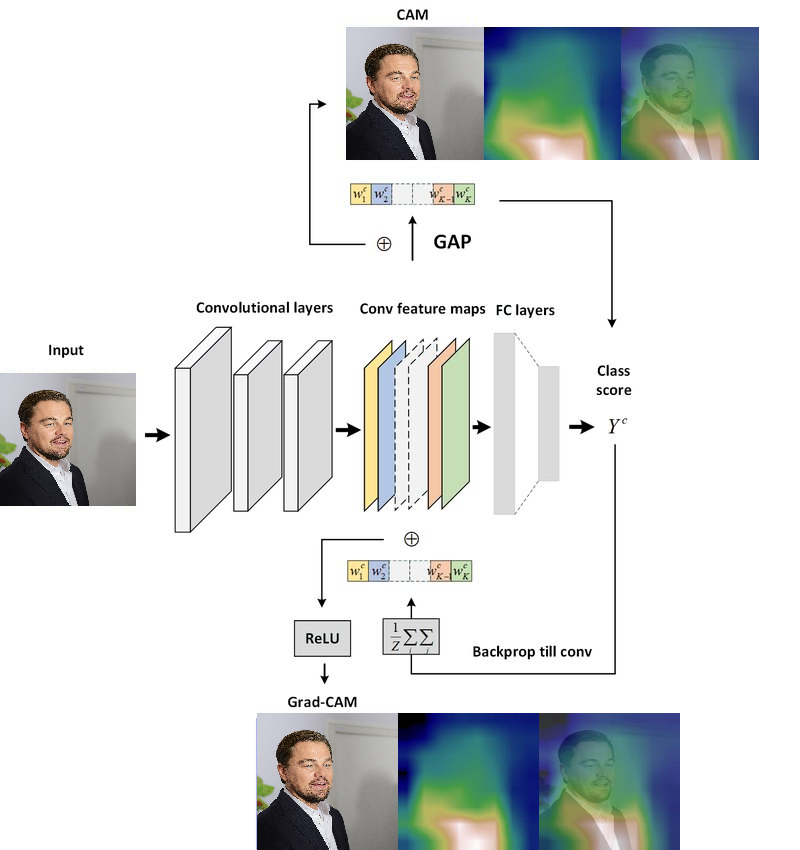
\includegraphics[width=0.60\textwidth]{gradcam_input.png}
    \caption{Esquema de mapeamento de ativação de classe (CAM/Grad-CAM) em uma rede
    convolucional: as ativações das últimas camadas convolucionais são combinadas para produzir
    um mapa de calor que evidencia as regiões mais influentes na decisão do modelo. Em trabalhos
    futuros, essa interpretabilidade será empregada para auditar se arquiteturas profundas (CNNs e
    ViTs) atendem a regiões anatomicamente plausíveis da íris, em vez de artefatos de aquisição.}
    \label{fig:gradcam}
    {\footnotesize Fonte: adaptado de \citet{selvaraju2017gradcam}.}
\end{figure}



% ====================== Referências ======================
\newpage
\begin{thebibliography}{99}

\bibitem[Anap et~al.(2025)]{AnapEtAl2025ICEC2NT}
Anap, M.; Bongulwar, M.; Chaskar, U.
\newblock Conventional Neural Network and Support Vector Machine for the Detection of Diabetes Mellitus.
\newblock \emph{2025 International Conference on Electronics and Computing, Communication Networking Automation Technologies (ICEC2NT)}, p. 1--8, 2025.

\bibitem[Australian Government(2025)]{AusGovIridology2025}
Australian Government Department of Health and Aged Care.
\newblock Iridology evidence evaluation: Appendices A--H (final), 2025.
\newblock Disponível em: \url{https://www.health.gov.au/sites/default/files/2025-03/02_iridology_appendices_a-h_final.pdf}

\bibitem[Deck(1981)]{Deck1981}
Deck, J.
\newblock \emph{Iris Diagnosis and Treatment}.
\newblock Thorsons Publishers, 1981.

\bibitem[Dosovitskiy et~al.(2021)]{dosovitskiy2021vit}
Dosovitskiy, A.; Beyer, L.; Kolesnikov, A.; Weissenborn, D.; Zhai, X.; Unterthiner, T.; Dehghani, M.; Minderer, M.; Heigold, G.; Gelly, S.; Uszkoreit, J.; Houlsby, N.
\newblock An image is worth 16x16 words: Transformers for image recognition at scale.
\newblock In: \emph{International Conference on Learning Representations (ICLR)}, 2021.

\bibitem[Ernst(2000)]{Ernst2000ArchOphthalmol}
Ernst, E.
\newblock Iridology: a systematic review.
\newblock \emph{Archives of Ophthalmology}, 118(1):120--121, 2000.

\bibitem[Gonzalez e Woods(2018)]{GonzalezWoods2018}
Gonzalez, R. C.; Woods, R. E.
\newblock \emph{Digital Image Processing}.
\newblock 4. ed.
\newblock Pearson, 2018.

\bibitem[Haralick et al.(1973)]{Haralick1973Texture}
Haralick, R. M.; Shanmugam, K.; Dinstein, I.
\newblock Textural features for image classification.
\newblock \emph{IEEE Transactions on Systems, Man, and Cybernetics}, v. 3, n. 6, p. 610--621, 1973.
\newblock doi: 10.1109/TSMC.1973.4309314.

\bibitem[He et~al.(2016)]{he2016resnet}
He, K.; Zhang, X.; Ren, S.; Sun, J.
\newblock Deep residual learning for image recognition.
\newblock In: \emph{IEEE Conference on Computer Vision and Pattern Recognition (CVPR)}, 2016, p. 770--778.
\newblock doi: 10.1109/CVPR.2016.90.

\bibitem[Jensen(1982)]{Jensen1982}
Jensen, B.
\newblock \emph{Science and Practice of Iridology}.
\newblock Bernard Jensen International, 1982.

\bibitem[Knipschild(1988)]{Knipschild1988BMJ}
Knipschild, P.
\newblock Looking for gall bladder disease in the patient's iris.
\newblock \emph{BMJ}, 297(6663):1578--1581, 1988.

\bibitem[Liu et~al.(2021)]{liu2021swin}
Liu, Z.; Lin, Y.; Cao, Y.; Hu, H.; Wei, Y.; Zhang, Z.; Lin, S.; Guo, B.
\newblock Swin Transformer: Hierarchical vision transformer using shifted windows.
\newblock In: \emph{IEEE/CVF International Conference on Computer Vision (ICCV)}, 2021, p. 10012--10022.

\bibitem[M{\"u}nstedt et~al.(2005)]{Munstedt2005JACM}
M{\"u}nstedt, K., El-Safadi, S., Br{\"u}ck, F., Zygmunt, M., Hackethal, A., Tinneberg, H.-R.
\newblock Can iridology detect susceptibility to cancer? A prospective case-controlled study.
\newblock \emph{Journal of Alternative and Complementary Medicine}, 11(3):515--519, 2005.

\bibitem[Ojala et al.(2002)]{Ojala2002LBP}
Ojala, T.; Pietik\"ainen, M.; M\"aenp\"a\"a, T.
\newblock Multiresolution gray-scale and rotation invariant texture classification with local binary patterns.
\newblock \emph{IEEE Transactions on Pattern Analysis and Machine Intelligence}, v. 24, n. 7, p. 971--987, 2002.
\newblock doi: 10.1109/TPAMI.2002.1017623.

\bibitem[OpenCV(2026a)]{OpenCVHistEq}
OpenCV.
\newblock Histogram Equalization.
\newblock \emph{OpenCV Documentation}, versão 4.x, acesso em 27 fev. 2026.
\newblock Disponível em: \url{https://docs.opencv.org/4.x/d4/d1b/tutorial_histogram_equalization.html}

\bibitem[OpenCV(2026b)]{OpenCVSmoothing}
OpenCV.
\newblock Smoothing Images.
\newblock \emph{OpenCV Documentation}, versão 4.x, acesso em 27 fev. 2026.
\newblock Disponível em: \url{https://docs.opencv.org/4.x/d4/d13/tutorial_py_filtering.html}

\bibitem[{{\"O}nal} et~al.(2022)]{OnalEtAl2022MTA}
{\"O}nal, M. N.; G{\"u}raksin, G. E.; Duman, Re\c{s}at.
\newblock Convolutional neural network-based diabetes diagnostic system via iridology technique.
\newblock \emph{Multimedia Tools and Applications}, 82(1):173--194, 2022.

\bibitem[Samant e Agarwal(2018)]{SamantAgarwal2018CMPB}
Samant, P., Agarwal, R.
\newblock Machine learning techniques for medical diagnosis of diabetes using iris images.
\newblock \emph{Computer Methods and Programs in Biomedicine}, 157:121--128, 2018.

\bibitem[Selvaraju et~al.(2017)]{selvaraju2017gradcam}
Selvaraju, R. R.; Cogswell, M.; Das, A.; Vedantam, R.; Parikh, D.; Batra, D.
\newblock Grad-CAM: Visual explanations from deep networks via gradient-based localization.
\newblock In: \emph{IEEE International Conference on Computer Vision (ICCV)}, 2017, p. 618--626.
\newblock doi: 10.1109/ICCV.2017.74.

\bibitem[Simon et~al.(1979)]{Simon1979JAMA}
Simon, A., Worthen, D. M., Mitas, J. A.
\newblock An evaluation of iridology.
\newblock \emph{JAMA}, 242(13):1385--1389, 1979.

\bibitem[Sruthi et~al.(2022)]{SruthiEtAl2022IJPRAI}
Sruthi, K.; Vijayakumar, J.; Thavamani, S.
\newblock Deep Learning-Based Verification of Iridology in Diagnosing Type II Diabetes Mellitus.
\newblock \emph{International Journal of Pattern Recognition and Artificial Intelligence}, 36(11), 2022.

\bibitem[Taghiyev et~al.(2024)]{TaghiyevEtAl2024AICT}
Taghiyev, F.; Mammadli, A.; Guliyeva, L.; Al-Dayyeni, W. S.
\newblock Diabetes Detection Based on Iridology.
\newblock \emph{2024 IEEE 18th International Conference on Application of Information and Communication Technologies (AICT)}, p. 1--11, 2024.

\bibitem[Touvron et~al.(2021)]{touvron2021deit}
Touvron, H.; Cord, M.; Douze, M.; Massa, F.; Sablayrolles, A.; J\'egou, H.
\newblock Training data-efficient image transformers \& distillation through attention.
\newblock In: \emph{International Conference on Machine Learning (ICML)}, 2021, p. 10347--10357.

\bibitem[Vaswani et~al.(2017)]{vaswani2017attention}
Vaswani, A.; Shazeer, N.; Parmar, N.; Uszkoreit, J.; Jones, L.; Gomez, A. N.; Kaiser, {\L}.; Polosukhin, I.
\newblock Attention is all you need.
\newblock In: \emph{Advances in Neural Information Processing Systems (NeurIPS)}, 2017, p. 5998--6008.

\bibitem[WHO(2024)]{WHOdiabetes2024}
World Health Organization (WHO).
\newblock Diabetes (Fact sheet), 2024.
\newblock Disponível em: \url{https://www.who.int/news-room/fact-sheets/detail/diabetes}

\bibitem[Zech et~al.(2018)]{Zech2018}
Zech, J. R., Badgeley, M. A., Liu, M., Costa, A. B., Titano, J. J., Oermann, E. K.
\newblock Variable generalization performance of a deep learning model to detect pneumonia in chest radiographs: A cross-sectional study.
\newblock \emph{PLOS Medicine}, 15(11):e1002683, 2018.

\bibitem[Zuiderveld(1994)]{Zuiderveld1994CLAHE}
Zuiderveld, K. J.
\newblock Contrast Limited Adaptive Histogram Equalization.
\newblock In: Heckbert, P. S. (ed.).
\newblock \emph{Graphics Gems}.
\newblock Elsevier, 1994, p. 474--485.

\end{thebibliography}

\end{document}
